%% jnuthesis 文档类的可选参数有:
%%   nobackinfo 取消封二页导师签名信息.注意,按照南大的规定,是需要签名页的.
%%   phd/master/bachelor 选择博士/硕士/学士论文

% 使用 blindtext 宏包自动生成章节文字
% 这仅仅是用于生成样例文档,正式论文中一般用不到该宏包
\documentclass[bachelor,adobefonts]{jnuthesis}

% 本科课程设计课程名称
\usepackage{graphicx}
\usepackage{subcaption}
\usepackage{algorithm}
\usepackage{algorithmic} 
\usepackage{amsmath}  


\renewcommand{\algorithmicrequire}{\textbf{Input:}} 
\renewcommand{\algorithmicensure}{\textbf{Output:}}


\graphicspath{ {images/} }
%%%%%%%%%%%%%%%%%%%%%%%%%%%%%%%%%%%%%%%%%%%%%%%%%%%%%%%%%%%%%%%%%%%%%%%%%%%%%%%
% 设置论文的中文封面

% 如果论文标题过长,可以分两行,第一行用\titlea{}定义,第二行用\titleb{}定义,将上面的\title{}注释掉
\titlea{复杂网络技术在数据挖掘中的应}
\titleb{用}



% 论文作者姓名
\author{汪建海}
% 论文作者学生证号
\studentnum{1030414623}
% 导师姓名职称
\supervisor{方伟}
\supervisorpos{副教授}
% 第二行导师姓名职称,仿照第一行填写,没有则留空
\supervisorb{}
\supervisorbpos{}
% 论文作者的学科与专业方向
\major{计算机科学与技术}
% 论文作者所在院系的中文名称,学士学位论文此处不带“学院”二字
\department{物联网工程}
% 论文作者所在学校或机构的名称.此属性可选,默认值为``江南大学''.
\institute{江南大学}
% 学士学位获得日期,需设置年、月,默认为编译日期.
\bachelordegreeyear{2018}
\bachelordegreemonth{6}
%%%%%%%%%%%%%%%%%%%%%%%%%%%%%%%%%%%%%%%%%%%%%%%%%%%%%%%%%%%%%%%%%%%%%%%%%%%%%%%

%-------------------------------------------------------------------------------
%	CODE INCLUSION CONFIGURATION
%-------------------------------------------------------------------------------
\usepackage{listings}
\newfontfamily\menlo{Menlo}
\usepackage{color}
\lstset{
    columns=fixed,,
    breaklines=true,
    % numbers=left,                                        % 在左侧显示行号
    % frame=single,                                        % 显示背景边框
    backgroundcolor=\color[RGB]{245,245,244},            % 设定背景颜色
    % keywordstyle=\color[RGB]{40,40,255},                 % 设定关键字颜色
    numberstyle=\footnotesize\color{darkgray},           % 设定行号格式
    commentstyle=\color[RGB]{0,96,96},                   % 设置代码注释的格式
    stringstyle=\color[RGB]{128,0,0},                    % 设置字符串格式
    showstringspaces=true,                              % 不显示字符串中的空格
    basicstyle=\small\menlo,
    numberstyle=\scriptsize\menlo,
    xleftmargin=0cm,
    xrightmargin=0cm
}

\begin{document}

%%%%%%%%%%%%%%%%%%%%%%%%%%%%%%%%%%%%%%%%%%%%%%%%%%%%%%%%%%%%%%%%%%%%%%%%%%%%%%%

% 制作中文封面
\maketitle

%%%%%%%%%%%%%%%%%%%%%%%%%%%%%%%%%%%%%%%%%%%%%%%%%%%%%%%%%%%%%%%%%%%%%%%%%%%%%%%
% % 开始前言部分
% \frontmatter

%%%%%%%%%%%%%%%%%%%%%%%%%%%%%%%%%%%%%%%%%%%%%%%%%%%%%%%%%%%%%%%%%%%%%%%%%%%%%%%
% 论文的中文摘要
\begin{abstract}
目前,数据挖掘和机器学习领域正在面临新的挑战,
因为收集和需要处理的信息量很大.
许多复杂的学习方法不能简单地处理庞大而复杂的领域,因为执行时间难以管理
,或者当领域变得更加复杂时发生的预测和通用性能力的丧失.
因此,为了应对当前现实世界问题的信息量,需要推进复杂数据挖掘技术的界限.

数据聚类是数据挖掘领域亟待研究重点与难点,对其研究在理论上和实际应用上都有重要的意义.
随着社交网络的崛起,比如新浪微博、知乎等网站蕴含着巨大的信息量,从大量的数据中挖掘有用的信息是一件极其不简单的事情.
近年来,很多领域都应用到了数据挖掘,比如金融的风险投资、广告精准投放、预测用户的购买行为等
,数据挖掘为人们的生活提供了巨大的便利,也创造了巨大的经济和社会价值.

通过对复杂网络的研究,人们可以量化和预测模糊世界,
而且能够在一定范围内预测事物的发展和运作,并能够预测网络崩溃. 
目前有大量实际可用的模型,并且这些模型已经在实际生产和组织结构中的大量应用中使用,并取得了大量的实际成果.

本文对知乎用户资料进行数据挖掘,采用Scrapy框架对数据进行有效的数据采集,
并应用知乎API采集特定的信息进行简单数据可视化.
通过复杂网络的的相关理论知识,结合特定应用领域的具体特性,
对特定应用领域的复杂网络特性进行分析研究.
利用特定应用的数据相互关系,
通过计算用户间关系相异度,并采用聚类算法和社团发现算法,
对数据之间的关系进行分析,得出数据实体的关系聚类图,
分析方法的实际效果. 


% 中文关键词.关键词之间用中文全角分号隔开,末尾无标点符号.
\keywords{数据挖掘;数据聚类; 复杂网络;聚类算法;网络模型}
\end{abstract}

%%%%%%%%%%%%%%%%%%%%%%%%%%%%%%%%%%%%%%%%%%%%%%%%%%%%%%%%%%%%%%%%%%%%%%%%%%%%%%%
% 论文的英文摘要



\begin{englishabstract}
  Currently, the data mining and machine learning fields are facing new challenges because of the amount of information that is collected and needs processing. 
  Many sophisticated learning approaches cannot simply cope with large and complex domains, 
  because of the unmanageable execution times or the loss of prediction and generality capacities that occurs when the domains become more complex.
   Therefore, to cope with the volumes of information of the current realworld problems there is a need to push forward the boundaries of sophisticated data mining techniques. 

  Data clustering is a key and difficult point in the field of data mining, and its research has important significance in
  the theory and practical application.
  With the rise of social network, websites such as Sina Weibo and Zhihu have a huge amount of information, and 
  finding useful information from the amount of data is extremely difficult.
  In recent years, many fields have been applied to data mining, such as financial risk investment, accurate placement of advertisements, 
  and prediction of users' puchase behavior. 
  Data mining provides greate comvenience for people's lives and also creates greate economic and social value.

  Through the research on complex network, people can quantify and predict the fuzzy world. 
  At present, only the research results based on complex networks can predict the development and operation of things within a certain range, 
  and can predict the network crashes.

  At the same time, a large number of practically available models are prodeced during the process of research on complex networks,
  and these models have been used in a large number if application in actual production and organizational Structures,
  and a great deal of practical results have been achieved.

  This paper conducts data mining for user data and uses Scrapy Framwork for effective data collection. 
  It also uses ZHIHUAPI to collect specific information for simple data visualization.
  Through the relevant theoretical knowledge of complex networks, combined with the specific characteristics
  of specific application areas, the complex network characteristics of specific application areas are ananluzed and studied.
  Using the data relationshaip of specific applications, by caculating the dissimilarity between users, 
  and using clustering algorithm and community discovery algorithm, 
  the relationship between data is analyzed to obtain the relationship clustering diagram of data entities.
  





% 英文关键词.关键词之间用英文半角逗号隔开,末尾无符号.
\englishkeywords{Data mining; Data clustering; Complex network; Clustering Algorithm; Network model}
\end{englishabstract}

%%%%%%%%%%%%%%%%%%%%%%%%%%%%%%%%%%%%%%%%%%%%%%%%%%%%%%%%%%%%%%%%%%%%%%%%%%%%%%%
% 生成论文目次
\tableofcontents

%%%%%%%%%%%%%%%%%%%%%%%%%%%%%%%%%%%%%%%%%%%%%%%%%%%%%%%%%%%%%%%%%%%%%%%%%%%%%%%
% 开始正文部分
\mainmatter

%%%%%%%%%%%%%%%%%%%%%%%%%%%%%%%%%%%%%%%%%%%%%%%%%%%%%%%%%%%%%%%%%%%%%%%%%%%%%%%
% 学位论文的正文应以《绪论》作为第一章

%第一章绪论
\chapter{绪论}\label{chapter_introduction}
\section{选题背景与意义}
计算机和信息技术的广泛使用导致了从广泛的应用领域创建大量数据库\cite{Li2002Unsupervised}.
如果适当的知识发现机制被用于提取嵌入数据中的隐藏的但潜在有用的信息\cite{Ahmad2007A},   
那么这样庞大的数据库可以对未来的决策做出重大贡献. 

DM是提取数据丰富,不完整,模糊和随机的有用信息和知识的过程\cite{李佩2005Agent, Pan2006Incorporating, Qian2009A}.    
DM被定义为大型复杂数据集的自动或半自动探索性数据分析,可用于揭示数据中的模式和关系,并强调大型观测数据库\cite{Miller2015A}. 
  现代统计和计算技术被应用于这个问题,以便找到隐藏在大型数据库中的有用模式\cite{Tsantis2001Enhancing, Sharma2015An}.
为了发现隐藏的趋势和模式,DM使用了明确的知识库,复杂的分析技能和领域知识.
实际上,通过DM的趋势和模式形成的预测模型使分析师能够从现有数据中产生新的观察结果. 
 DM方法也可以被看作是统计计算,人工智能(AI)和数据库方法.
 但是,这些方法并没有取代现有的传统统计数据;实际上,它是传统技术的延伸.例如,其技术已被应用于发现隐藏的信息并预测金融市场的未来趋势. 
 DM在商业和金融方面取得的竞争优势包括增加收入,降低成本,提高市场反应和意识\cite{Zhang2004Discovering}.
 它也被用于推导新的信息,这些信息可以集成到决策支持,预测和估计中,以帮助企业获得竞争优势.  
 在高等教育机构中,DM可以用于发现隐藏的趋势和模式,帮助他们预测学生的成绩. 
 
% 数据挖掘(Data Mining,DM)又称数据库中的知识发现(Knowledge Discover in DataBase,KDD),是数据库中知识发现阶段之一.
% 涉及跨学科领域,如机器学习,人工智能,数据库理论和统计学等邻域.
% 数据挖掘的具体含义就是从大量的数据中,
% 去寻找有规律的、隐含在大量数据中的、并且对人们有价值的信息的过程.
% %数据挖掘就是从数据库中的大量数据中挖掘有效的信息,即从不完全的、模糊的、大量的、随机的
% %实际数据中,去发现有规律的、隐含的、有用的、人们事先未知的但却潜在有价值的并且最终可理解的信息和知识的非平凡过程.

% %数据挖掘是一种决策支持的过程,它主要基于人工智能、机器学习、模式识别、统计学、数据库、可视化技术等,
% %高度自动化第分析企业的数据,做出归纳性的推理,从中挖掘出潜在的模式,
% %帮助决策者调整市场策略,减少风险,做出正确的决策.
% 数据挖掘具体过程就是决策支持的过程,主要是帮助商业决策者去对公司数据进行高度自动化分析,做出可行性的归纳推理,
% 从而调整市场策略的过程,这样不仅可以帮助决策者减少风险,而且在可预测的范围内做出最佳的决策.

所以说对挖掘技术的研究必然可以提高有用信息的获取,
从而直接或间接推动这些应用的性能和实用性的提高,具有重要的研究意义和价值.

\section{数据挖掘的发展与现状}
\subsection{数据挖掘的历史及发展}

\begin{figure}[htp]
  \centering
  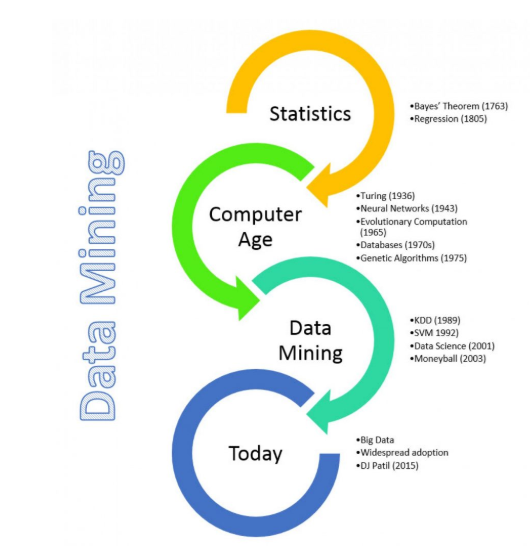
\includegraphics[width=0.6\linewidth]{shujufajuefazhan.png}
  \caption{数据挖掘发展历程}
\end{figure}

数据挖掘是一门有着悠久历史的学科,
它从早期的数据挖掘方法贝叶斯定理(1700年)\cite{邵金楠2017经典贝叶斯决策理论概述}
和回归分析(1800年)\cite{陈希孺1989最小一乘线性回归}开始,
这些分析主要是识别数据中的模式.从下面的时间顺序表中简要地看到数据挖掘历史的主要里程碑:


数据挖掘是从不同角度分析大数据集(大数据)的过程,
揭示相关性和模式以将其汇总为有用的信息.
现在它融合了许多技术,如人工智能,统计学,数据科学,数据库理论和机器学习等\cite{黄河燕2016大数据情报分析发展机遇及其挑战}.

技术的日益强大和数据集的复杂性使得数据挖掘公司从静态数据交付演变为更加动态和主动的信息交付;
从磁带和磁盘到高级算法和海量数据库.在80年代后期,统计学家,数据分析师和管理信息系统(MIS)社区开始了解和使用数据挖掘术语.
到了20世纪90年代初,数据挖掘被认为是一个子过程或者是一个称为数据库知识发现(KDD)的更大过程中的一个步骤, 这实际上使得它成为“受欢迎的人”.
 KDD最常用的定义是“识别数据中有效,新颖,潜在有用且最终可理解的模式的非平凡过程”(Fayyad,1996)\cite{Feyyad1996Fayyad}.
在过去的十年里,数据挖掘的普及率一直在迅速增长.

从20世纪70年代,数据挖掘技术主要经历了四个阶段,总结如图(1-1)所示:

\begin{figure}[htp]
  \centering
  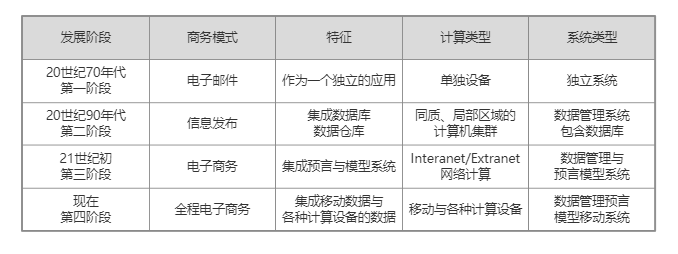
\includegraphics[width=1.0\linewidth]{Wsjwj.png}
  \caption{数据挖掘发展}
\end{figure}


\subsection{数据挖掘的研究现状}
目前我国在数据挖掘技术研究上已经取得了巨大的成果,
常用的数据挖掘模型包括神经网络模型、决策树模型、遗传算法模型、粗糙集模型、模糊集模型、关联规则模型等\cite{任新社2016关于数据挖掘研究现状及发展趋势的探究}.

近年来,数据挖掘取得的了很多最新研究成果,本文选择了四篇研究大数据挖掘领域的论文,
这些论文提供了数据挖掘领域的概述而且对未来该邻域进行广泛的概述.


(1)由\ Ryaboy\ 和\ Dmitriy\ 写的名为“Scaling Big Data Mining Infrastructure: The Twitter Experience”\cite{Ryaboy2013Scaling}的论文中介绍到:
有关大数据挖掘基础架构的见解,
以及在Twitter上进行分析的经验.它表明,由于数据挖掘工具的当前状态,执行分析并不简单.
大部分时间都用于数据挖掘方法应用的准备工作,并将初步模型转化为可靠的解决方案.

(2)由\ Yizhou\ Sun\  和\ Jiawei\ Han\ 写的名为“Mining Heterogeneous Information Networks: A
Structural Analysis Approach”\cite{Sun2012Mining}的论文中表明:
挖掘异构信息网络是大数据挖掘研究中一个新的有前景的研究前沿,
它将互连的多类型数据(包括典型的关系数据库数据)视为异构信息网络.
这些半结构化的异构信息网络模型利用网络中类型化节点和链接的丰富语义,
可以从互联数据中发现令人惊讶的丰富知识.

(3)由\ U\ Kang\ 和\ Christos\ Faloutsos\ 写的名为“Big graph mining:algorithms and discoveries”\cite{Kang2013Big}的论文中介绍了挖掘大图的概述,重点介绍了Pegasus工具的使用,并展示了Web Graph和Twitter社交网络中的一些发现.本文为大图挖掘提供了鼓舞人心的未来研究方向.

(4)由\ Xavier\ Amatriain\ 和\ Christos\ Faloutsos\ 写的名为“Mining Large Streams of User Data for Personalized
Recommendations”\cite{Amatriain2013Mining}的论文中介绍了Netflix奖学习的一些经验教训,
并讨论了Netflix中使用的推荐人和个性化技术.它讨论了最近的重要问题和未来的研究方向.
文中第4节包含了一个有趣的讨论,关于我们是否需要更多数据或更好的模型来改进我们的学习方法.

有关大数据挖掘中的其他重要工作可以在主要会议上找到,如KDD、ICDM、ECMLPKDD或期刊例如“数据挖掘和知识发现”或“机器学习”等.

\section{论文主要工作}
本文围绕研究将数据挖掘中的聚类知识与复杂网络有关模型进行有机融合,提出了基于复杂网络的数据挖掘的应用,
并就特定的用户数据进行研究,本文的主要工作有下面几个方面.

(1)通过查找文献了解复杂网络和数据挖掘的定义和具体实现方法,对现有相关研究做一定的综述工作.

(2)研究知乎用户数据并采用特定的方法对数据进行爬取,并对知乎用户数据进行简单的数据可视化.

(3)通过研究特定的聚类算法并实现,分析实习的效果并分析他的优缺点,并应用算法对数据进行聚类,分析聚类效果.

(4)用社团发现算法并结合复杂网络模型对数据进行分析,通过计算用户间关系相异度, 分析数据以获得数据关系聚类图,分析方法的实际效果.

\section{论文结构安排}
本论文总共分为五个章节,每个章节的内容概括如下:

(1)第一章为绪论,首先介绍了课题的研究背景,然后介绍了该数据挖掘领域中的历史发展和研究现状,
并且简单描述了本文的研究内容,最后给出了全文的结构安排.

(2)第二章对复杂网络的相关知识进行的说明,介绍复杂网络的网络特性和网络模型.

(3)第三章介绍数据抓取的细节,并对数据做出一些清洗,为后文提供数据.

(4)第四章为聚类算法的研究,详细说明了算法的实现的具体细节并分析实现效果,说明了算法的优缺点,
并用复杂网络技术对数据进行聚类分析.

(5)第五章为结论与展望,对本文主要工作进行了总结,对存在的不足进行了展望.





\chapter{复杂网络}
我们在现实生活中经常发现你的朋友的朋友可能也是你的朋友,
现实生活中很多网络表现除了很强的聚类性,尤其是社交网络.
社交网络是一组人或一群人,他们之间有一些互动模式或“关系”.一群人之间的由友谊,
公司之间的业务关系以及家庭的通婚都是过去研究过的网络例子.
所以本章节主要介绍有关复杂网络的基本理论和体现网络特征的参数,为后面章节打下了坚实的理论基础.

\section{复杂网络的定义}
复杂网络是由节点和节点之间许多复杂连接组成的网络结构,它是通过边连接的节点组成,
节点可以任意分配一定的信息的网络系统的基本单元,边则是表示基本单元之间的关系或着相互作用.
% 复杂网络是由数量巨大的节点和节点之间错综复杂的关系共同构成的网络结构,
% 它是由大量的节点通过边的相互连接而构成的图,其中的节点可以是任意具有特定动力和信息
% 内涵的系统的基本单元,边则表示基本单位之间的关系或相互作用.

但是,到目前为止,复杂网络还没有统一的定义,复杂网络一般具有以下特征:
(1)它是大量真是系统的拓扑抽象;
(2)它的统计特征介于规则网络和随机网络之间.
钱学森给\cite{钱学森1990一个科学新领域——开放的复杂巨系统及其方法论}出了复杂网络一个较严格的定义:

\begin{definition}  
  具有自组织、自相似、吸引子、小世界、无标度中部分或全部性质的网络成为复杂网络(Complex neworks).  
\end{definition} 

复杂网络简而言之即呈现高度复杂性的网络.其复杂性主要表现在一下几个方面:
\textcircled{1} 结构复杂:体现在巨大的节点数量,复杂的网络结构;
\textcircled{2} 网络进化:体现在节点或者节点之间的连接与消失;
\textcircled{3} 连接多样性:节点之间的边的权重不一样,而且边具有不同的方向;
\textcircled{4} 动力学复杂性:数据节点集属于非线性动力学系统;
\textcircled{5} 节点多样性:复杂网络中的节点可以代表任何事物;
\textcircled{6} 多重复杂性融合:就是以上几点之间的交互,将会导致更加不可预测的结果

在数学上,网络用图(Graph)来表示,所以不需要关心节点的位置,
边的长度和形状,只需要关心节点之间是否相连接.

% \begin{definition}  
%   一个图 $G = (V,E)$是一个二元组,这个二元组包括一个节点集V,一个边集E.
%   $|V|$表示节点的总数,$|E|$表示边的总数.图中节点的总数和边的总数分别称为图的阶和规模.
% \end{definition} 

% 按照边是否有方向可以分为有向图和无向图:

% \begin{definition}  
%   如果在一个图$G$,边$x \rightarrow y$ 与边 $y \rightarrow x$ 要么同时存在,
%   要么不存在,把这两条边合为一条边记为$xy$或$yx$,这样的图叫做无向图(Undirected network),
%   否则称为有向图(Directed network).
% \end{definition} 

% 按照边的权重,图可以分为无权图和加权图:

% \begin{definition}  
%   对于图$G(V,E)$,如果对于任意的边有$|e_i| = 1$,则称$G$为无权图(Unweighted network),
%   否则则称为加权图(Weighted network).
% \end{definition} 


\section{复杂网络的网络特征}
\subsection{网络概述}
节点的度简单说就是与该节点相连边的个数.

\begin{figure}[h!]
  \centering
  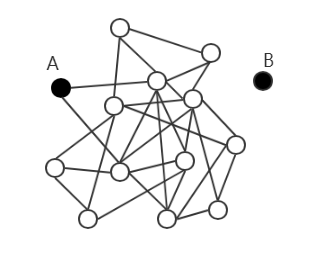
\includegraphics[width=0.6\linewidth]{Wwuxiangtu.png}
  \caption{节点度的示意图}
\end{figure}

在图2-1中,复杂网络中度为0的节点称为孤立节点.
如图2-1所示是一个无向图,节点A的度数为2,节点B为一个孤立节点.

一个节点最简单最重要的局部特征就是节点的度,网络中所有节点度的平均值称为网络的平均度,
用$P_k$来表示:

\begin{equation}
P_k= \frac{1}{N} \sum_{v \in V}^{}d(v).
\end{equation}
式中中$\sum_{v \in V}^{}d(v)$表示所有节点度数之和.

平均加权度是在统计节点度是,同时也考虑边的权重.可以简单理解为在平均度的计算中,将边的权重全为当作1来计算,
而在计算平均加权度的时候则是要根据实际的边的权重计算节点的度,并根据加权的度来计算平均的度.

网络中节点度值分布特征是网络的重要几何性质,
度分布(Degree distribution)是用来体现网络中节点度分布状况的函数,一般用$P(k)$表示.

在规则网络中,每个节点都有相同的度数,用$k_0$表示每个节点的度数,则其网络度分布服从$\delta$分布,如图2-2所示:

\begin{equation}
  P(k) = \delta_0(k) = 
  \left\{
    \begin{array}{lr}
      1, & k = k_0,\\
      0, & k\neq k_0.
    \end{array}
  \right.
\end{equation}

在随机网络\cite{Erdos1959On}中,度分布服从泊松分布,如下图2-2所示:
\begin{figure}[h!]
  \centering
  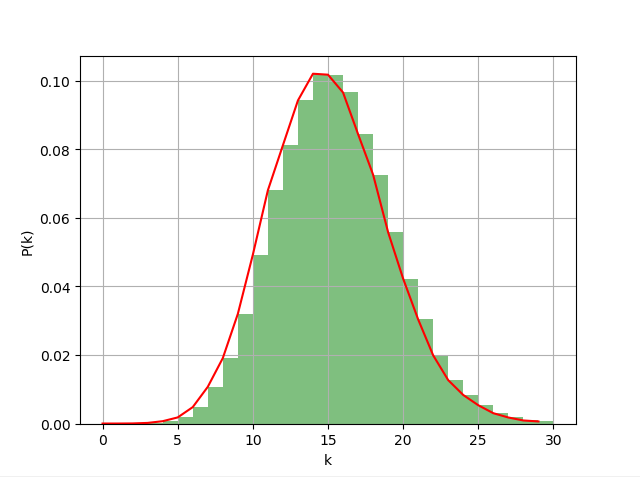
\includegraphics[width=0.6\linewidth]{Wposong.png}
  \caption{泊松分布}
\end{figure}

但是Barabási和Albertlászló等人\cite{Barab1999Emergence}人研究了一个包含325739节点的万维网子网,
他们通过实验发现发现万维网的度分布不像规则网络和小世界网络\cite{Watts1998Collective, Newman2000Mean}那样是对称的泊松分布,
而是幂律分布(Power law distribution).
如图2-3所示为幂律分布函数图,从这个图中可以很容易地看出,随着k的增加,曲线中没有出现峰值,
而且还可以从图中看出较多的节点度数很小,
极个别的节点度数很高(这些节点我们成为中枢点),
并且网络中的节点具有很强的异质性.


\begin{figure}[h!]
  \centering
    \begin{subfigure}[b]{0.4\linewidth}
      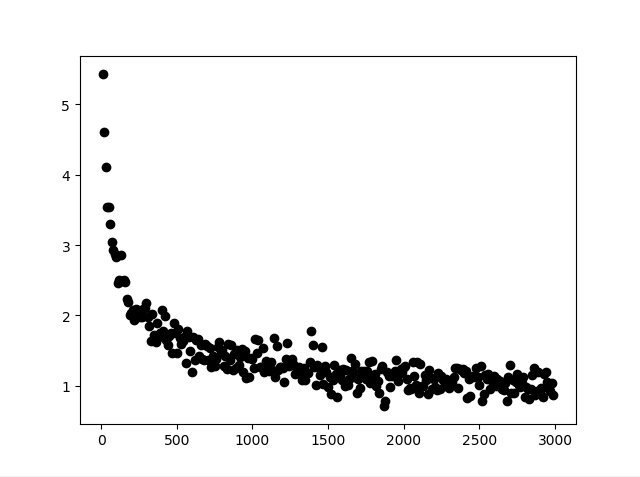
\includegraphics[width=\linewidth]{Wmilv.png}
      \caption{}
    \end{subfigure}
    \begin{subfigure}[b]{0.4\linewidth}
      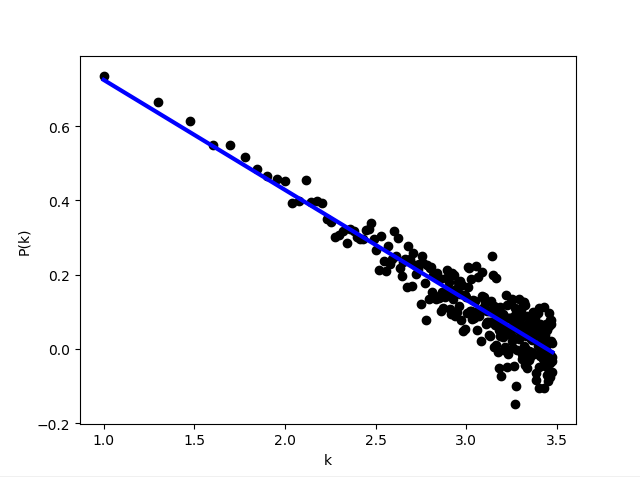
\includegraphics[width=\linewidth]{WmilvN.png}
      \caption{}
    \end{subfigure}
  \caption{幂律分布}
\end{figure}


网络中的度分布\cite{Kong2012Markov, Hou2009Degree}是否遵循松分布或幂律分布关键取决于网络中的节点是反映同质还是异质.
与此同时还可以确认网络的性质,我们从数学关系上可以简单的知道指数函数是半对数坐标系中的一条直线,
而幂律分布在双对数坐标系中是直线.
因此,为了确认度分布函数之间的确切关系只需要在半对数或者双对数坐标系绘制分布函数,即可简单的区分开它们.

% 网络度分布服从泊松分布还是幂律分布,反映了网络中节点之间是同质或异质的,
% 进而可以分析网络的很多性质.指数函数在半对数坐标系中是一条直线,
% 而幂律分布在双对数坐标系中是一条直线,因此为了区分度分布函数是指数衰减还是幂律衰减的,
% 我么只需要把度分布函数在半对数或双对数坐标系中划出其图像,通过观察即可区别开.

网络直径是统计的边的连接特性,统计网络直径后,得出的值是一个网络整体的.模块化是根据图的连接关系对节点做归类,
类型相同的节点会增加一个字段,用相同的数字表示.模块化在社会学中可以用于社区发现.
\subsection{节点概述}
聚类系数(Clustering coeffocient)\cite{kaiser2008mean}是指一个节点一度连接的节点中,实际的边数与最大边数之比.
% 实验结果证明显示,在现实世界的网络中,尤其在特定的网络中,
% 由于相对高密度连接点的关系,节点总是去向建立一组严密的组织.
% 在现实世界的网络,这种可能性往往比这两个节点但之间随机设立了一个连接的平均概率要大.
聚类系数的定义如下:
% \begin{definition}
  % 计算节点$v_i$的聚集系数,假设A节点的度数为$k_i$,那么在它的邻域最多有$C_{k_i(N)}^{2} = \frac{k_i(N)(k_i(N)-1)}{2}$条边.
  % 节点A的聚类系数为:
  \begin{equation}
    C_i = \frac{d_1}{C_{k_i}^{2}} = \frac{2d_1}{k_i(k_i-1)}
  \end{equation} 
式子中,$d_i$表示与节点A相连的节点数目,$C_{k_i}^{2}$表示与A节点相连节点之间最大的连接数目.

  网络的平均聚类系数(图中所有节点聚类系数的平均值):

  \begin{equation}
    C = \frac{1}{N}\sum_{i = 1}^{N}C_i.
  \end{equation}
% \end{definition}
式子中,节点总数表示为N.

计算过程如下:
\begin{figure}[h!]
  \centering
  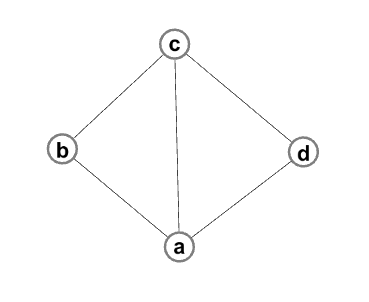
\includegraphics[width=0.6\linewidth]{juleixishu.png}
  \caption{聚类系数}
\end{figure}
计算节点a的聚类系数,图中a节点度为1的节点有b、c、d, 这三条节点只有两条边(b-c,c-d),而这三个节点之间最多可以有3条边(b-c,c-d,d-b).
因此a节点的聚类系数约为0.67,同理可得节点b、c、d的聚类系数为1.00,0.67,1.00,故该图的平均聚类系数为(1.00*2+0.67*2)/4=0.8333.

特征向量中心度\cite{spizzirri2011justification}也是能够表示节点重要性的一个参数.
核心节点不仅与大量的其他节点相连,而且也会与其他重要的核心节点相连,这是特征向量中心度的主要思想.
% 核心思想是一个重要节点不仅与其他许多节点有连接,而且与其它相连的节点也是比较重要的节点.
特征向量对于有向网络和无向网络都适用,在无向网络效果更好,但在有向网络中使用,否则讨论特征向量中心度是没有意义的.

% \begin{equation}
%   C = \sum_{i=1}^{N}C_i \frac{C_{k_i(N)}^{2}}{\sum_{j=1}^{N}C_{k_j(N)}^{2}}
%     = \frac{\sum_{j=1}^{N}E(i)}{\sum_{j=1}^{N}C_{k_j(N)}^{2}}
% \end{equation}

% \begin{definition}
% 首先计算网络三个连通节点的总数,然后计算网络中三角形的总数,网络的聚类系数定义为:
%   \begin{equation}
%     C = \frac{3 \times \text{三角形的总数}}{\text{网络中三个连通节点的总数}}.
%   \end{equation}
% \end{definition}

% 简单的理解聚类系数就是指一个节点的节点中,实际边数与最大边数之比.
% 例子就是网络数据可视化与分析利器Gephi中文教程P185.理解聚类系数和平均聚类系数.


\subsection{边概述}
描述边的特性一共有三个,分别是最短路径、网络直径、平均路径长度.其中最短路径是指在一个网络中,两个节点连接最短的路径;
最短路径的值就是最短路径中边的个数.在复杂网络中,所有最短路径的最大值就是网络直径;
所有网络最短路径之和的平均值等于这个网络的平均路径长度,这两个特性是整个网络的指标.


\begin{definition}  
  \textbf{平均最短路径长度:} 指一个网络中,节点的数量除以所有两个节点最短路径之和,记为$d_a$.
\end{definition} 
\begin{equation}
    d_a = \frac{1}{\frac{N(N-1)}{2}}\sum_{i \leq N}\sum_{j > i}d_{(i,j)}.
\end{equation}
其中i,j表示为网络中的两个节点,并定义节点i到自身的距离为0.
% 平均最短路径长度也可以理解为求平均每个最短路径 可以分配到几个节点.




这里以图2-5(a)中节点2到节点1的路径为例,在节点2与节点1之间共有两条路径可以连通,
第一条是:$2 \rightarrow 3 \rightarrow 4 \rightarrow 5 \rightarrow 1$;
第二条是:$2 \rightarrow 3  \rightarrow 5 \rightarrow 1$.
第二条路径短,所以最短路径就是第二条,数量为3.图2-5(b)中所示可以看出节点1到节点2的值最大(为3),
网络直径也就是3.由图2-5(c)和图2-5(d)可以得出最短路径长度为16/10=1.6.

\begin{figure}[h!]
  \centering
    \begin{subfigure}[b]{0.49\linewidth}
      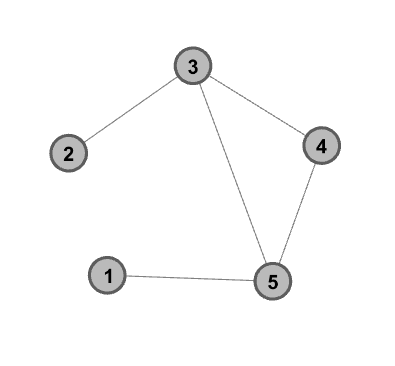
\includegraphics[width=\linewidth]{biantexing.png}
      \caption{网络边}
    \end{subfigure}
    \begin{subfigure}[b]{0.49\linewidth}
      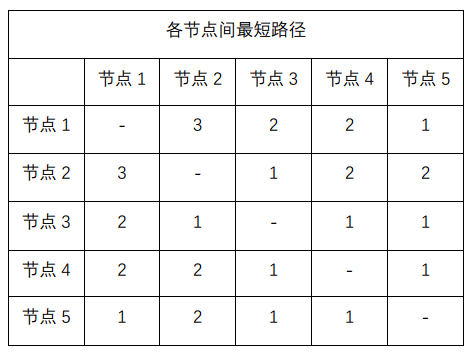
\includegraphics[width=\linewidth]{bian1.png}
      \caption{最短路径}
    \end{subfigure}
    \begin{subfigure}[b]{0.49\linewidth}
      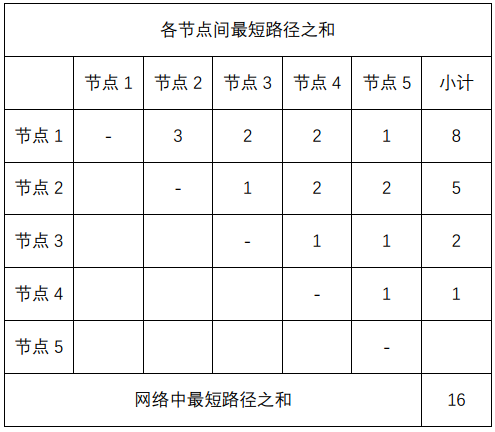
\includegraphics[width=\linewidth]{bian2.png}
      \caption{最短路径之和}
    \end{subfigure}
    \begin{subfigure}[b]{0.49\linewidth}
      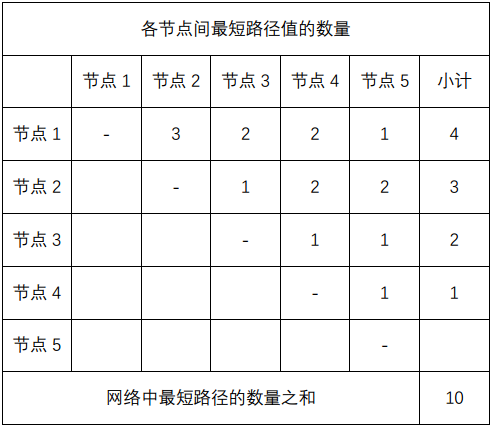
\includegraphics[width=\linewidth]{bian3.png}
      \caption{最短路径的数量}
    \end{subfigure}
  \caption{边特性}
\end{figure}






\section{复杂网络模型}
\subsection{随机网络模型}
% 随机网络就是如果节点不按照确定的规则连接,而是以一定的概率连接,所得的网络.
20世纪60年代,随机网络模型由埃德加·纳尔逊·吉尔伯特(Edgar Nelson Gilbert,1923-2013)\cite{Gilbert1959Random}独立介绍,
同年匈牙利数学家Erdos和Renyi发表了他们的第一篇论文提出了ER随机网络模型\cite{Erdos1959On}.
然而,Erdős和Rényi的作品的影响如此之大以至于他们被正确地视为随机图论的创始人.
最简单的随机网络模型是Erdös-Rényi随机网络(ER随机网络),其中所有边都是独立的.

对于ER随机网络有两种生成机制,
一种是G(N,L)模型, N个标记的节点与L个随机放置的链接链接.
Erdős和Rényi在他们的随机网络论文中使用了这个定义\cite{Erdos1959On, Erd2012On}.
如图2-6(a)所示.
另一种是G(N,P), 对于节点总数为N的网络,任意两个节点之间的连接概率为p.
这是Gilbert引入的一个模型\cite{Gilbert1959Random}.如图2-6(b)所示.
两种机制的关系是$L=p \times \frac{N(N-1)}{2}$,$p=\frac{2L}{N(N-1)}$.

% 推导过程:

% 对于ER随机网络模型有两种不同的生成机制.
% (1)给定网络节点总数N,网络中任意两个节点以概率$p$连线,生成的网络全体记为$G(N,p)$,
% 构成一个概率空间.由于网络中连接数目是一个随机变量$X$,取值可以从0到$\frac{N(N-1)}{2}$,
% 有$n$条连线的网络数目为$C_{\frac{N(N-1)}{2}}^{n}$,
% 其中一个特定网络出现的概率为$P(G_n) = p^n(1-p)^{\frac{N(N-1)}{2} - n}$.
% 因此可生成不同的网络总数为$2^{\frac{N(N-1)}{2}}$,它服从二项分布.
% 网络中节点的平均连线数为$p\frac{N(N-1)}{2}$.

% (2)给定网络节点总数N,随机连接网络中的n条边,
% 而这些连线是从总共$\frac{N(N-1)}{2}$条可能的连线中随机选取的,
% 生成网络全体记为$G(N,n)$,构成一个概率空间.这样生成的不同网络的总数为$C_{\frac{N(N-1)}{2}}^{n}$,
% 它们出现的概率相同,服从均匀分布,网络中两个节点连线的概率为$\frac{2n}{N(N-1)}$.


\begin{figure}[h!]
  \centering 
  \begin{subfigure}[b]{0.49\linewidth}
    \centering
    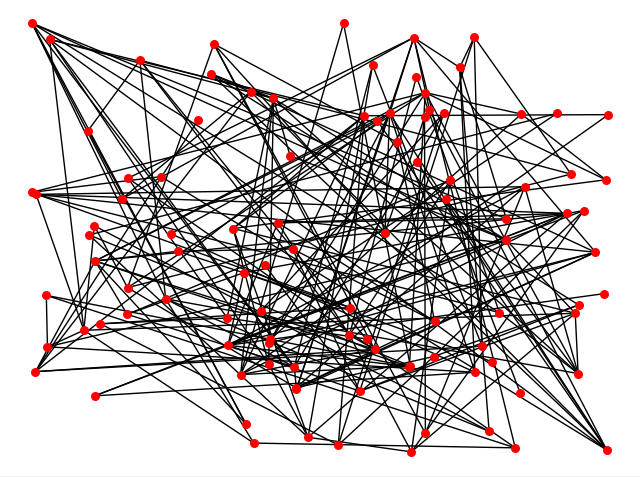
\includegraphics[width=\linewidth]{WER-4.png}
    \caption{N = 100,L = 200}
  \end{subfigure}
  \begin{subfigure}[b]{0.49\linewidth}
    \centering
    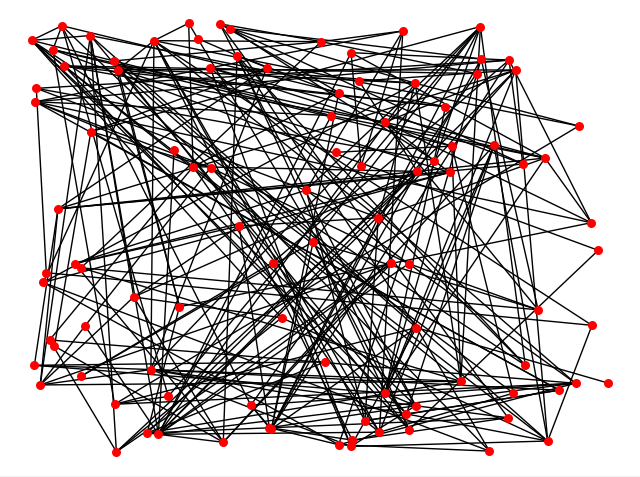
\includegraphics[width=\linewidth]{WER-2.png}
    \caption{N=100,P=0.05}
  \end{subfigure}
  \caption{随机网络模型}
\end{figure}

图2-6(a)中的,节点数为100,边数为200,两个节点连接概率为0.0404;平均度和平均加权度都为1.99(因为每条边的加权值都为1,和平均度值一样),
网络直径为7,图密度为0.04,平均聚类系数为0.025,迭代100次的网络特征向量中心度为0.01405,
平均路径长度为3.392.图2-6(b)中,节点数为100,两节点连接概率为0.05,边数为269;平均度和平均加权度为2.69,网络直径为6,
图密度为0.027,平均聚类系数为0.047,迭代100次的网络特征向量中心度为0.00553,
平均路径长度为2.84.




% 如图2-4(a)所示是一个具有50个节点,节点之间的连接概率为$p = 0.1$的ER随机网络.
% 网络中的节点平均度数为$<k> = 4.8$,网络的聚类系数为$C = 0.1068$.
% 如图2-4(b)所示是一个具有100个节点,节点之间的连接概率为$p = 0.0.05$的ER随机网络.
% 网络中的节点平均度数为$<k> = 4.98$,网络的聚类系数为$C = 0.03735$.

% \begin{figure}[h!]
%   \centering 
%   \begin{subfigure}[b]{0.49\linewidth}
%     \centering
%     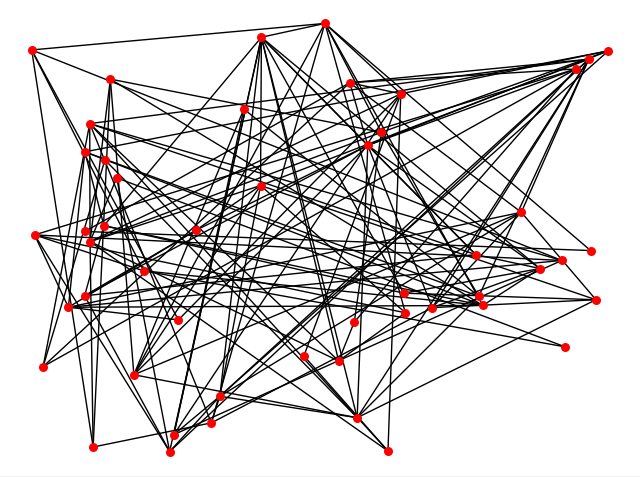
\includegraphics[width=\linewidth]{WER-1.png}
%     \caption{N=50,p=0.1}
%   \end{subfigure}
%   \begin{subfigure}[b]{0.49\linewidth}
%     \centering
%     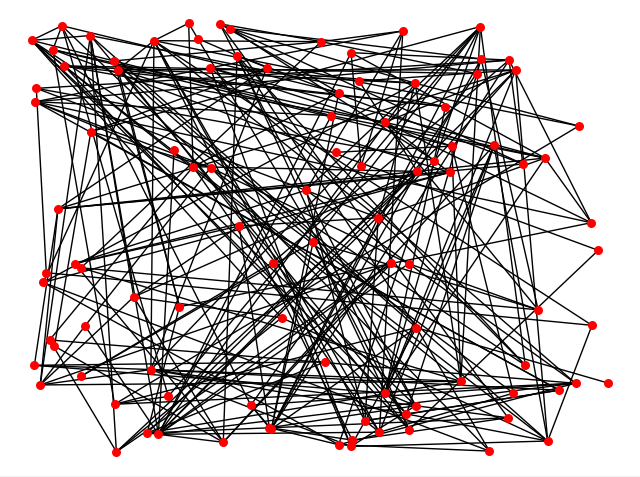
\includegraphics[width=\linewidth]{WER-2.png}
%     \caption{N=100,p=0.05}
%   \end{subfigure}
%   \caption{第一种机制生成ER随机网络模型}
% \end{figure}




% \begin{figure}[h!]
%   \centering 
%   \begin{subfigure}[b]{0.49\linewidth}
%     \centering
%     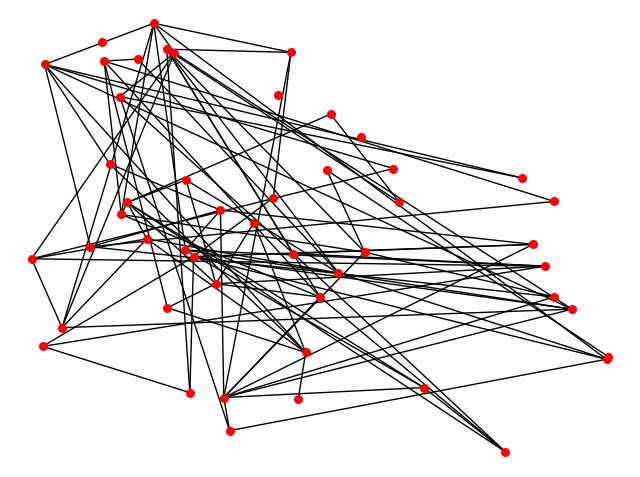
\includegraphics[width=\linewidth]{WER-3.png}
%     \caption{N = 100,m = 100}
%   \end{subfigure}
%   \begin{subfigure}[b]{0.49\linewidth}
%     \centering
%     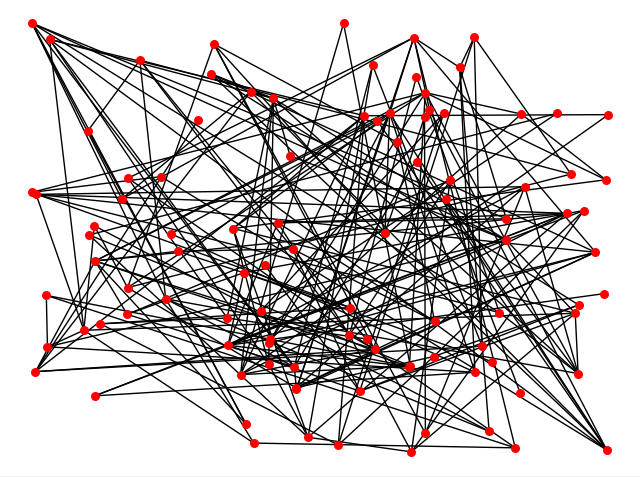
\includegraphics[width=\linewidth]{WER-4.png}
%     \caption{N = 100,m = 200}
%   \end{subfigure}
%   \caption{第二种机制生成ER随机网络模型}
% \end{figure}


% 如图2-5(a)所示是一个具有50个节点,100条连线的ER随机网络.
% 网络中的节点平均度数为$<k> = 3.96$,网络的聚类系数为$C = 0.08092$.
% 如图2-5(b)所示是一个具有100个节点,200条连线的ER随机网络.
% 网络中的节点平均度数为$<k> = 4.06$,网络的聚类系数为$C = 0.07368$.


% 对于ER随机网络的两种生成机制,
% 当$p\frac{N(N-1)}{2} = n$时,模型$G(N,p)$和$F(N,n)$是等价的.
% 当网络中的节点数N比较大时,ER随机网络的节点度分布可以近似为泊松分布,
% 由于网络中存在大量的随机连线,网络的聚类系数比较小.

\subsection{小世界网络模型}

小世界现象,也被称为六度分离,
长期以来一直令广大公众着迷.
它指出,如果你选择地球上任何地方的任何两个人,
你会发现他们之间至多有六个熟人的路径.
居住在同一个城市的个人只有几次握手的事实并不令人意外.
小世界网络是许多现实世界网络的两个属性是任何节点对之间的距离相对较小,同时传递性或聚类的水平相对较高.
小世界的概念指出,即使是地球另一端的个人也可以通过一些熟人与我们联系.

在1998年,\ Duncan\ Watts\ 和\ Steven\  Strogatz\ 提出了随机网络模型的扩展\cite{Watts1998Collectivedynamics}:
(1)小世界属性:
在实际网络中,两个节点之间的平均距离取决于N的对数关系,而不是遵循正则格的期望多项式. 
(2)高聚类:对于类似的N和L的随机网络,实际网络的平均聚类系数远高于预期.

Watt和Strogatz开发了一个模型,
将网格模型的传递性与随机网络模型的低路径长度相结合,
创建了一个称为小世界网络的模型.
他们从具有高聚类和高平均路径长度的晶格模型开始.
然后,向模型中添加概率p边缘重新布线,意味着边缘与其中一个节点断开连接,
然后随机连接到网络中任何位置的另一个节点.选择每个边缘以概率独立重新布线p.

% 当发生概率 p很低,
% 那么大多数连接仍然是它们连接网格中附近节点的原始本地连接.
% 出于这个原因,传递性仍然很高.
% 然而,已经重新布线的一些边缘可能会变成长距离连接,以连接格子中彼此远离的节点.
% 这些长距离连接或快捷方式立即在快捷方式任一端周围的节点之间创建一个短距离.
% 这个结论隐含了这样一个事实,即路径长度将每个边缘计为一个长度,
% 因此即使我们经常将它们绘制为长连接,快捷连接也只会在路径长度上添加一个.

\begin{figure}[h!]
  \centering
  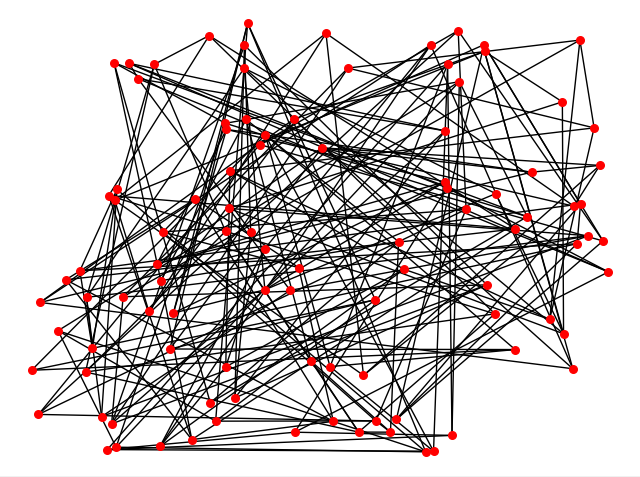
\includegraphics[width=0.6\linewidth]{WWS.png}
  \caption{WS小世界网络模型(N=100,K=4,p=0.04)}
\end{figure}

如图2-6所示节点总数为100,节点与邻近四个节点相连接,连接概率为0.04的WS模型.
平均度为4,网络的聚类系数为0.4127.

Watts-Strogatz模型(也称为小世界模型)重新生成高聚类和小世界现象共存.
作为随机网络模型的扩展,WattsStrogatz模型预测了一个类似泊松的有界度分布.
理解高聚类的小世界属性的共存必须从网络的正确度分布开始.
% 是一个具有100节点,每个节点与最近邻的4个邻居相连,重连概率为0.04的WS小世界网络模型.
% 网络中节点的平均度$<k> = 4$,网络的聚类系数$C = 0.4127$.


% 通过研究发现,规则网络具有比较大的聚类系数,
% 但随着网络规模的增大,它的平均路径长度也很大;
% 而对于随机网络,虽然它有较小的平均路径长度,但其聚类系数也很小.
% 为了更好的发现实际网络的内在机制,Watts和Strogatz在1998年提出了小世界模型.
% WS小世界网络模型的生成机制如下:

% (1)初始:给定一个具有N个节点的环,
% 环上每个节点都与它最邻近的K=2k个节点但相连,构成一个最近邻环网络.

% (2)重连:以概率p对环网中的每条连线进行重新连线,方法是将选择的每条连线的一端断开,
% 然后随机的连接到其他的节点桑,不允许自连线和重复连线.

% 通过最近网络随机重连得到的WS小世界网络模型的很多性质介于规则网络和随机网络之间,
% 通过调节重连概率p可以实现从规则网络p=1到随机网络p=1的过度.
% 由于在规则网络中进行重连,使得网络中存在随机的连线,形成捷径,
% 从而网络中节点间的最短路径长度大大减少.
% 由此我们可以看出WS小世界网络模型具有较小的平均路径长度和较大的聚类系 数.




\subsection{BA无标度网络模型}
现实世界网络的一个共同特征是中枢节点或与网络中其他节点高度连接的少数节点.
中枢点的存在会给度分布一个长尾巴,表示中枢点的个数很少但度数却很高,而大部分节点度数少但个数且很多.

1999年,当\ Barabasi\ 和\ Albert\ 在研究万维网的时候发现,万维网的都度分布不符合随机网络和WS模型,
因而提出了BA网络模型\cite{Albert2002Statistical}(也就是无标度网络模型).无标度网络模型符合幂率分布.
% 1999年,Barabasi和Albert在研究万维网时发现,万维网的度分布不想随机网络和小世界
% 那样具有对称的泊松分布,而是偏倚的幂律分布.在该网络中,大多数节点仅有少量连线,
% 而少数节点拥有大量的连线.为此他们提出了无标度(scale-free)网络模型,
% 揭示了增长和择优机制在复杂网络自组织演化过程中的普遍性和幂律的重要性.
% BA无标度网络模型的生成机制如下:

% (1)初始:开始时给定一个含有$n_0$节点以一定的规则连接的网络;

% (2)增长:在每个时间步增加一个带有$m(m \leq n_0)$条信赖年界限的新节点;

% (3)择优:新节点以择优概率

% \begin{equation}
%   \prod (k_i) = \frac{k_i}{\sum_{j}^{}},
% \end{equation}
% 选择旧节点i与之连线,其中$k_i$世界点i的度数.

% 这个模型提出了两条重要的网络演化机制:增长和择优,这是从万维网实际形成过程中抽象出来的,
% 万维网每时每刻都有新的网页增加.增长和择优是生成无标度网络不可缺少的内在机制.
% 无标度网络中的节点具有异质性,不同度的节点在网络中的重要程度不同.
% 在社会网络中,都可以表示个体的作用力和影响都,一个点的度越大,
% 一般表示在整个网络系统组织中的作用和影响越大,反之亦然.

% \begin{figure}[h!]
%   \centering 
%   \begin{subfigure}[b]{0.49\linewidth}
%     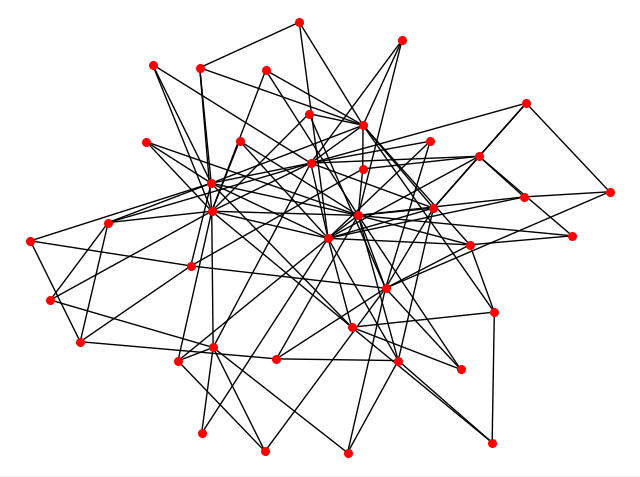
\includegraphics[width=\linewidth]{WBA-1.png}
%     \caption{N=40,m=3}
%   \end{subfigure}
%   \begin{subfigure}[b]{0.49\linewidth}
%     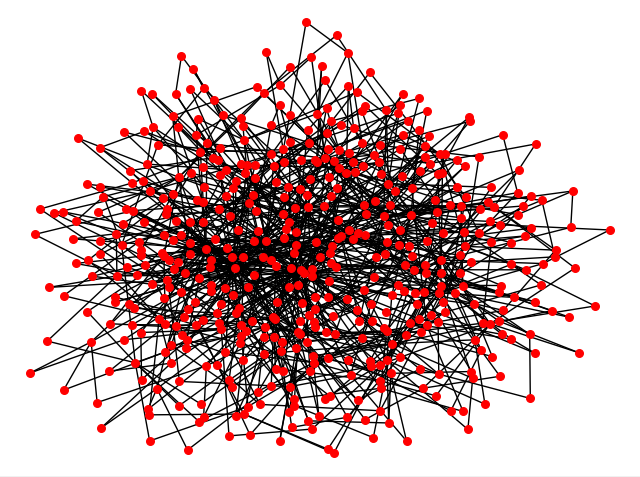
\includegraphics[width=\linewidth]{WBA-2.png}
%     \caption{N=500,m=2}
%   \end{subfigure}
%   \caption{BA无标度网络模型}
% \end{figure}

% 如图2-7(a)所示是一个具有40个节点,每个节点新加入的节点带有3条新连接线的BA无标度网络模型.
% 网络中的节点平均度数为$<k> = 5.55$,网络的聚类系数为$C = 0.2993$.
% 如图2-7(b)所示是一个具有500个节点,每个节点新加入的节点带有2条新连接线的BA无标度网络模型.
% 网络中的节点平均度数为$<k> = 3.984$,网络的聚类系数为$C = 0.03618$.

% BA无标度网络模型的度分布严格服从指数为3的幂律分布,
% 当网络规模较大时,网络具有较小的平均路径长度,但是网络的聚类系数也比较小.
% BA无标度网络模型可以魔术一大类实际的网络,揭示了增长和择优时长生无标度的内在机制.








无标度网络模型(scale-free model)是一种以高度数中枢点为特征的网络模型,其度分布符合幂率分布,可以将其度分布写为:
\begin{equation}
  P_d(k) \propto k^{-\gamma}
\end{equation}
式中$\gamma $是指数,度分布$P_d(k)$随着度数k的增减而衰减越来越缓慢,增加了找到非常大程度的节点的可能性.


\begin{figure}[h!]
  \centering
  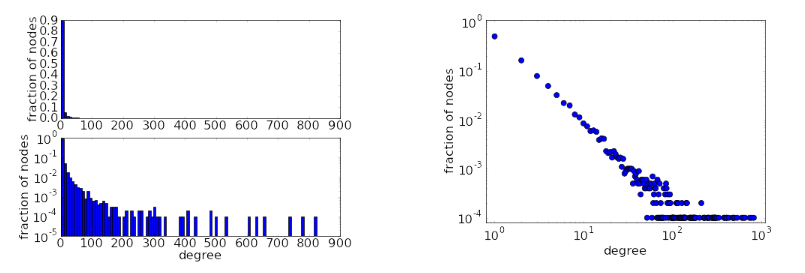
\includegraphics[width=1\linewidth]{BAmoxing.png}
  \caption{BA模型}
\end{figure}
图2-8说明了节点数目为10000,幂律指数$\gamma =2$的无标度网络的度分布,其平均度大约为7,
但是3/4的节点的度数小于等于3,在第一个条形图中,看不见有大于100度的节点,但用第二个中绘制条形高度会显示度分布的长尾.
尽管大多数节点的度数很少,但是有几个节点度数可以超过500,这些中枢点的度数数量级比大多数节点的数量级要大,这就是幂律网络的一个特点.
我们可以清楚的看到,度分布绘制在双对数坐标上,散点图将倾向于沿着一条直线下落,这也是幂律分布的特点.









% \subsection{其他网络模型}





% 当然除了本章节所介绍的三种网络模型以外,还有其他模型,
% 比如Bollobas提出的LCD(Linearized chord diagrams)模型、
% Liu等人提出的混合连接网络模型以及Zhang等人提出的广义的合作网络(两者都属于具有随机和则有连线规则的网络模型)、
% Holme和Kim提出的HK网络模型都能够描述一大类网络特性,本文就不再继续介绍相关知识,有兴趣的可以查阅资料了解.















% \section{复杂网络度分布的求解方法}
% \subsection{平均场方法}
% Barabasi等人为了分析BA模型的度提出了平均场方法(mean-field approach).
% 具体步骤如下:



% 令$k_i(t)$表示节点$i$(在第i时刻加入到网络的节点)在时刻t的度数,
% 对于BA模型,
% 在t时刻网络共增加了m条线,每条线连接网络中的两个节点,
% 此时网络中节点的读书之和$\sum_{i}^{}k_i(t)\approx 2mt$.
% 根据连续性理论,把$k_i(t)$看作连续动力学函数,则$k_i(t)$满足如下的动力学方程:

% \begin{equation}
%   \frac{\partial k_i(t)}{\partial t} = 
%   m\prod (k_i(t)) = \frac{k_i(t)}{2t}
% \end{equation}

% $$k_i(t) = m.$$
% 上述方程有如下解:
% \begin{equation}
%   k_i(t) = m\left( \frac{t}{t} \right)^{1/2}.
% \end{equation}
% 由于节点是随机选择的,因此$i$在所有节点中服从均匀分布,
% 又初始网络中含有$n_0$个节点,从而$\rho (i) = \frac{1}{t+n_0}$.由式(2-10),可得

% \begin{equation}
%   P\{k_i(t)<k\} = P\left\{ i>\frac{m^2t}{k^2}\right\}
%   = 1-\frac{m^2}{k^2(t+m_0)},
% \end{equation}
% 对$k$求导即可得到$P(k,t)$:
% ($P(k,t)$表示在时刻t的度数为k的节点所占比例)

% \begin{equation}
%   P\{k_i(t)<k\} = \frac{\partial P\{k_i(t)<k\}}{\partial k} = 
%   2m^2k^{-3}\frac{t}{t+n_0}
% \end{equation}
% 当$t \rightarrow \infty$时,网络稳态分布为:

% \begin{equation}
%   P\{k\} = \lim_{t \rightarrow \infty} P\{k_i(t)<k\} \propto 2m^2k^{-\lambda}
% \end{equation}
% 其中,$\lambda =3$为标度指数,$k_i(t)$表示节点$i$在时刻t的度数,$m$表示在$t$时刻增加的连线.

% 通过平均场方法得出BA模型的度分布服从指数为3的幂律分布.

% \subsection{率方程方法}
% Krapivsky等人在分析网络度分布时提出了率方程方法(rate-equation approach),
% 率方程方法的求解如下:
% 令$N_k(t)$在t时刻网络中的度数为$k$的节点的总数,
% 对于BA模型,
% $\sum_{k}^{}kN_k(t)\approx 2mt.$
% 根据连续性理论,现在考虑节点数的变化率,
% 对于原来度数为$k-1$的节点由于与新节点但相连度数变为$k$,需要算入,
% 对于原来度数为$k$的节点,由于增加了连线度数变为$k+1$,需要排除;对于新节点,
% 它的度数恰好为$m$,若$k=m$,则需要保留.
% 节点与新加入的节点相连的概率为
% $m \frac{k_i(t)}{\sum_{k}^{}N_k(t)}$,
% 可得到关于$N_k(t)$的率方程:
% \begin{equation}
%  \frac{dN_k(t)}{dt} = N_{k-1}(t)\frac{k-1}{\sum_{k'}^{}k'N_{k'}(t)} - N_k(t)m
%  \frac{k}{\sum_{k'}^{}k'N_{k'}(t)} + \delta_{k,m}.
% \end{equation}
% 由大数定律得
% $$\lim_{t \rightarrow \infty}E\left( \frac{N_k(t)}{t}\right) = P(k)$$
% 式(2-12),可表示为
% \begin{equation}
%   (k+2)P(k) = (k-1)P(k-1) + 2\delta_{k,m}.
%  \end{equation}
%  式(2-13)是一个关于P(k)的一阶差分方程,解此差分方程可得:
%  \begin{equation}
%   P(k) = \frac{2m(m+1)}{k(k+1)(k+2)} \propto 2m^2k^{-3}.
%  \end{equation}
% 其中$N_k(t)$表示在t时刻网络中的度数为$k$的节点的总数

%  通过率路方法得到的BA模型的度分布服从3的幂律分布,此结果与用平均场方法所得结果一致.

% \subsection{其他方法}
% Bollobas等人用靶方法严格证明了LCD模型度分布的存在行并求出了度的表达式:

% \begin{equation}
%   \lim_{t \rightarrow \infty}P(k,t) = P(k).
% \end{equation}

% 侯振挺等人在BA模型应用马氏链理论的首达概率及其方法和技巧,
% 给出了网络度分布的精确表达式如下:

% \begin{equation}
%   P(k) = \frac{2m(m+1)}{k(k+1)(k+2)}
%   \propto2m(m+1)k^-3
% \end{equation}

% 马氏链方法在求解复杂网络度分布中,具有一定的普适性,
% 他们对增长网络和演化网络的度分布进行了系统的分析,
% 对增长网络、混合网络和演化网络的度分布问题给出一个统一的解答.

% 这些方法就不再给出详细的证明过程,只给出一些结论.有兴趣的可以查阅资料了解相关内容.






\chapter{用户信息采集}
如果要对用户关系之间的网络进行分析,首先就要对用户信息进行采集.
本章节将介绍知乎用户的采集采集过程,以及采集特定数据的方法,并对数据进行简单的可视化工作.

\section{网站选取}
知乎是一个中国消费者的平台,其产品形态与Quora(美国一家问答网站)并无二致,知乎用户可以提出问题并可以从数据库中接受答案以及获取其他用户的答案。
该平台从2011年1月26日创建,截至2017年9月份,知乎官方宣布知乎注册用户超过1亿人次,其中每天知乎有2600万用户至少花费1个小时时间在知乎平台上浏览,
月浏览量高达180亿次点击。知乎气氛浓厚,其内容得到广泛认可和信赖。基于用户、话题和其他元素,平台上的高质量内容可以快速传播到其他相关社区。
“有问题请知乎”是总结知乎平台的最佳句子.其凭借高质量的内容,知乎在互联网信息发布过程中的信息达到了上游位置。

知乎用户的主要特点是收入高、消费能力强、学历高等。其中本科及以上学历的用户占比80.1\%,中高收入和小康用户是知乎的主要人群,占比76.0\%.
这些知识渊博的人利用他们的批判性思维技能来分享他们在各个邻域的知识,从而创建一个具有社会认可度强大的“个性化品牌”。
当人们越来越依赖专业人员的帮助和建议时,这些专业人员时创造热门话题和影响他人决策的关键。知乎注册用户破亿是知乎平台的一个里程碑,在这样的环境下
知乎网站应该进一步从用户主体、用户体验、界面优化和使用规则等各个方面进行改善,进而构建一个全民的知识性的平台。

知乎尽管不进行新闻报道,但是知乎也可以成为关注的焦点,比如魏则西事件,雷洋事件、豫章事件等;发布在知乎上的内容,大家都可以分享,评论和发表个人的看法,
能够推动事件的发展;另外知乎算法更加倾向于专家给出的答案,而且专业也会相互评论和相互交流看法,增加了网站的影响力和可信度。
这说明知乎越来越具有影响力,在巨大的信息量面前必定隐藏了丰富的内容和有用的价值,因此对知乎的信息挖掘是有意义的。

% 据腾讯新闻报道:“知乎是一家创立于2011年1月26日的中国大陆社会化问答网站,产品形态模仿了美国类似网站Quora;
% 2012年2月底,知乎使用‘发现更大的世界’作为其宣传口号; 
% 截至2017年9月20日,知乎宣布注册用户数超1亿 ,
% 日活跃用户量达2600万,人均日访问时长1小时,月浏览量180亿; 
% 全站目前累计产生了1300万个问题,4600万个回答及3500万赞同”.

% 根据艾瑞 2017 年知乎用户调查报告,“知乎用户具有高学历和高消费能力等特点.
% 其中,知乎本科及以上用户占比 80.1\%,中高收入及小康用户是知乎主力人群,占比 76.0\%;
% 知乎称用户破亿是知乎从社区迈向平台的里程碑.在此背景下,
% 知乎进一步加速构建知识平台,从用户主体、使用场景、平台规则和工具功能等各个层面进行完善”.

% 《经济学人》认为“在中国网络审查的环境下,知乎出人意料地成为了政治讨论的发起点;
% 尽管知乎并不提供新闻报道,但有时知乎也会掀起风波,成为焦点;例如魏则西事件、豫章书院事件;
% 发布在知乎上的问题有时候能够推动事情的发展,如雷洋事件等.知乎的算法会倾向于专家给出的答案,
% 专家也会经常互相校正、评论,增加了网站的可信度.”
% 这也在一定程度上说明了知乎具有越来越大的影响力.知乎里面蕴含着巨大的信息量,
% 同时也隐藏着巨大的价值,因此对知乎信息的挖掘是有意义的.

\section{实验环境}
\subsection{环境搭建}
数据爬取的实验环境如下表3-1所示:
\begin{table}[h!]
  \centering\begin{tabular}{clcl}
    \toprule
    \textbf{类别} & \textbf{描述} & \textbf{类别}  & \textbf{描述}\\
    \midrule
    开发语言  &  Python3.6       & 开发框架  &  Scrapy1.5\\
    操作系统  &  Windows10 pro   & 系统环境  &  Anaconda4.5\\
    CPU型号   &  Intel i5-4210M  & 内存大小  & 4GB\\
    \bottomrule
  \end{tabular}
  \caption{实验环境}
\end{table}

\subsection{框架介绍}
本文采集知乎用户信息用的$Scrapy$框架,
$Scrapy$是一个用$Python$实现的开源并可以免费使用的跨平台的网络爬虫框架,
它主要目的是为爬取网络提供支持;并支持$JSON$、$CSV$、$XMl$等多种格式输出;
具有内置支持,通过$XPATH$或$CSS$表达提取源代码;支持一步并自动爬取数据;
易扩展、爬取高效、程序健壮等优点

$Scrapy$于2008年6月2日首次发布,截至2018年3月,最新版本为$Scrapy$为1.5版本且与$Python3.6$兼容.
目前有许多公司比如$CareerBuilder$,$DayWatch$,$PriceWiki$和$Tarlabs$等都在使用$Scrapy$作为爬取网站的框架.

$Scrapy$是一个集成系统,
包括一个控制所有组件之间数据流的引擎(\href{https://doc.scrapy.org/en/latest/topics/spiders.html}{$Scrapy Engine$}),
一个接收请求的调度程序(\href{https://doc.scrapy.org/en/latest/}{$Scheduler$}),
一个获取网页的下载程序(\href{https://doc.scrapy.org/en/latest/topics/downloader-middleware.html}{$Downloader middlewares$}),
一个Spider中间件(\href{https://doc.scrapy.org/en/latest/topics/spider-middleware.html}{$Spider middlewares$}),
以及用户编写的用于解析响应(\href{https://doc.scrapy.org/en/latest/topics/items.html}{$Item Pipeline$})和
提取项目的自定义类(\href{https://doc.scrapy.org/en/latest/topics/spiders.html}{$Spiders$}).

从网页上捕获和抓取数据的任务常常分为两个不同的阶段来执行:爬行和任务的抓取部分.
对于抓取知乎用户的详细信息,$Scrapy$是一个不错的选择,因为它是一个基于$Python$的框架,提供了用于爬行和抓取数据的工具;
此外,$Scrapy$作为开源产品,拥有强大的社区并能够为用户提供有效的帮助.
接下来本文用图3-1展现$Scrapy$的架构,包括各种组件以及在系统中发生的数据流的展示(绿箭头).

\begin{figure}[h!]
  \centering
  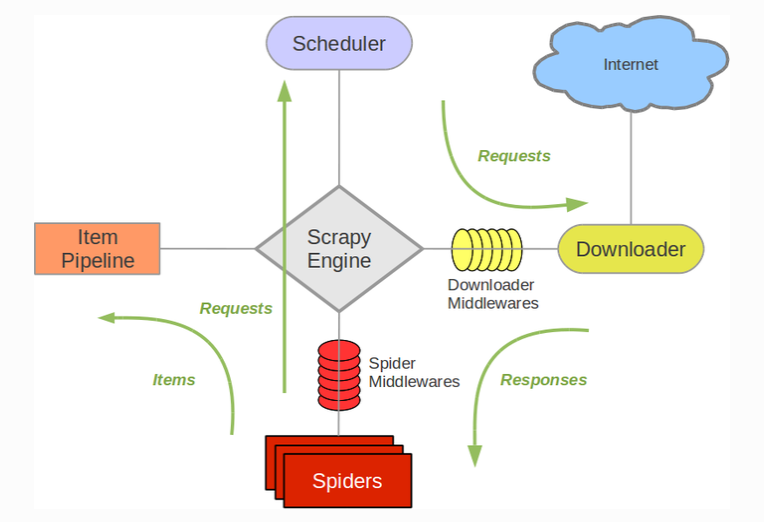
\includegraphics[width=0.8\linewidth]{Wscrapy.png}
  \caption{$Scrapy$框架}
\end{figure}

了解更多详细信息请参考
\textbf{\href{https://doc.scrapy.org/en/latest/}{官方文档}}


% 该框架具有:
% (1) 采用可读性更强的xpath代替正则;
% (2) 支持异步,同时在不同的url爬行;
% (3) 强大的统计和log系统;
% (4) 支持shell方式,方面独立调试;
% (5) 写middleware,反面写一些统一的过滤器;
% (6) 通过管道方式存入数据库.


\section{知乎用户详细资料抓取过程}
\subsection{采集流程}
下面给出本文采集数据的思路,如图3-2所示:

\begin{figure}[h!]
  \centering
  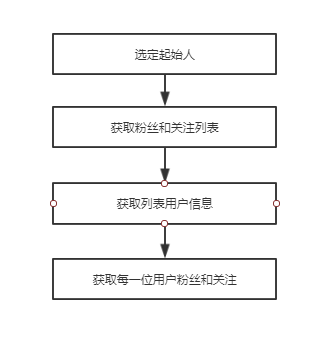
\includegraphics[width=0.4\linewidth]{Wsilu.png}
  \caption{设计思路}
\end{figure}

选定初始人就是选定以为关注数或者粉丝数多的大V作为爬取起始点.(本文选取的是$vczh$)
获取粉丝和关注列表就是通过知乎接口获得该大V的粉丝列表和关注列表.
获取列表用户信息就是通过知乎接口获得列表中每一位用户的详细信息.
(获取用户详细信息的链接是获取json格式的资料,这样不用加载其他资源,访问速度快),n是数据集中包含数据点的个数,
获取每一位用户粉丝和关注,进一步对列表中的每一个用户,获取他们的粉丝和关注列表,实现递归爬取.

下面列举一些采集过程中用的技巧,并列出本文在爬取时的参数(在项目中settings.py中可以设置):

\begin{lstlisting}
  # 可以提高下载速度,建议夜里设置为False,可以减少服务器负担
  ROBOTSTXT_OBEY = False  
  # 设置并发请求数量,默认16,为了提高CPU利用率,可以适当调节
  CONCURRENT_REQUESTS = 32
  # 设置网址禁止记录cookies可以提高CPU和内存利用率
  COOKIES_ENABLED = False
  # 设置日志级别,降低级别可以有利于提高性能
  LOG_LEVEL = 'INFO'
  # 设置禁止重试,当网站响应慢时可提高爬行效率
  RETRY_ENABLED = False
  # 设置下载超时,对于下载超时的网站,可以快速放弃该站点并释放资源
  DOWNLOAD_TIMEOUT = 15
  # 设置下载延迟,为了防止反爬虫,缓解服务器压力
  DOWNLOAD_DELAY = 0.25
  DOWNLOADER_MIDDLEWARES = {
    # 设置HTTP代理
    'scrapy.contrib.downloadermiddleware.httpproxy.HttpProxyMiddleware':543,
    # 设置高度可逆代理,为了防止知乎对IP限流,采用的时动态IP代理
     'zhihuuser.middlewares.ProxyMiddleware': 125,
    # 设置禁止本地记录浏览器用户代理,可以随机使用下面的用户代理
    'scrapy.downloadermiddlewares.useragent.UserAgentMiddleware': None,
    # 设置用户代理,模仿浏览器访问网站,可以有效的反爬虫
    'zhihuuser.middlewares.ZhihuuserUser_agentMiddleware': 126,
}
\end{lstlisting}

% (1)增加并发,并发是指同时处理的request的数量,其有全局限制和局部(每个网站)限制.
% Scrapy并发增加的程度取决于您的爬虫能占用多少CPU.
%  一般开始可以设置\quad $CONCURRENT\_REQUESTS = 100$ .为了优化性能,您应该选择一个能使CPU占用率在80\%-90\%的并发数.

% (2)禁止cookies\quad $COOKIES\_ENABLED = False$ ,能减少CPU使用率及Scrapy在内存中记录轨迹,提高性能.

% (3)降低log级别\quad $LOG\_LEVEL = 'INFO'$ ,可以减少CPU使用率及记录log存储的要求,在进行爬取使用INFO log级别.
% 在开发的时候可以使用DEBUG来显示你想要的信息.

% (4)禁止重试\quad $RETRY\_ENABLED = False$ ,提高对失败的HTTP请求进行重试会减慢爬取的效率,尤其当站点响应很慢时.

% (5)减小下载超时\quad $DOWNLOAD\_TIMEOUT = 15$ ,能让卡住的连接能被快速的放弃并解放处理其他站点的能力.

% 本文还采用了scrapy的反爬技巧,例如知乎网站对IP流量有限制,

% (1) 使用user-agent池,随机选择来作为user-agent.

% (2) 禁止cookies,站点会使用cookies来发现爬虫的轨迹.

% (3) 使用 Google cache 来爬取数据.

% (4) 使用动态IP代理池,每秒可获得5个IP.可以有效的躲过知乎的异常流量检测,对于知乎网站限制爬虫有很好的效果.

% (5) 使用高度分布式的下载器(downloader)来绕过禁止(ban),只需要专注分析处理页面.

为了提高爬虫速度还可以利用分布式爬取网站,只需要维护一个请求队列即可.
还有一些其他处理技巧,就不在一一列举具体的项目细节可以参考
\textbf{\href{https://github.com/Dcwjh/Scrapy_zhuhuuser}{zhihuuser}}

\subsection{爬取用户关注列表}
爬取用户的详细的关注列表或者时粉丝列表可以使用\href{http://zhihu-oauth.readthedocs.io/zh_CN/latest/index.html}{知乎API}
该框架的使用最重要的类就是ZhihuClinet,想要获取知乎的数据就就必须先创建ZhihuClinet对象并登录。

\begin{lstlisting}
  # 创建了ZhihuClient对象
  client = ZhihuClient()
  # 如果有token.pkl用户登陆记录可直接加载登陆资料,
  client.load_token('token.pkl')
  # 如果没有请登陆并保存登陆记录,请使用下面方法:
  try:
    client.login('email_or_phone', 'password')
  except NeedCaptchaException:
    # 保存验证码并提示输入,并登录
    with open('a.gif', 'wb') as f:
        f.write(client.get_captcha())
    captcha = input('please input captcha:')
    client.login('email_or_phone', 'password', captcha)
  # 上面可以简单一点写成:
  client.login_in_terminal('email@example.com', 'password')
  # 保存登陆记录
  client.save_token('token.pkl')
\end{lstlisting}

要想获取特定用户的粉丝或者关注列表就必须确定该用户的url\_token,
由于上节已经获取到了用户的详细资料中含有url\_token,本节就直接使用.
具体关键代码代码如下:
\begin{lstlisting}
  # 读取用户的id
  for line in open('url_token.txt'):
    line = f.readline()
    result.append(line.strip('\n'))
  f.close()
  # 获取关注列表并写入列表
  for p in result:
      try:
          people = client.people(p)
          f = open('following.txt', 'a')
          for following in people.followings:
              if following.over:
                  continue
              try:
                  f.write(people.name + ',' + following.name + '\n')
              except Exception as e:
                  continue
          f.close()
      except Exception as e:
          continue 
  print("finish")
\end{lstlisting}

\subsection{爬取数据及数据可视化}
爬取的知乎信息字段如下表3-2所示:

\begin{table}[h!]
  \centering\begin{tabular}{llllll}
    \toprule
    \textbf{Field} & \textbf{类型 } & \textbf{含义} & \textbf{Field} & \textbf{类型 } & \textbf{含义} \\
    \midrule
    \_id                       & Object  & 唯一标识用户    & name                       & String  & 用户名称\\
    gender                     & Int32   & 性别(1男,0女)   & deadline                   & String  & 用户一句话介绍 \\
    location                   & String  & 用户居住地      & educations                 & String  & 教育经历\\
    url\_token                 & String  & 用户表示字段    & answer\_count              & Int32   & 回答数目      \\ 
    thanked\_count             & Int32   & 获得感谢数目    &question\_count             & Int32   & 提出问题数目\\
    follower\_count            & Int32   & 粉丝数目        & artticles\_count           & Int32   & 文章数目     \\
    following\_count           & Int32   & 关注数目        & following\_topic\_count    & Int32   & 关注话题数目 \\
    following\_columns\_count  & Int32   & 关注专栏数目    & following\_question\_count & Int32   & 关注问题数目 \\ 
    \bottomrule
  \end{tabular}
  \caption{数据字段}
\end{table}

由于爬取的数据字段有50个,表3-2只列举常用字段.

本文爬取数据耗时6个小时共爬取数据35825条数据.
爬取用户粉丝列表如下格式:
\begin{table}[h!]
  \centering\begin{tabular}{llll}
    \toprule
    \textbf{用户} & \textbf{关注用户} & \textbf{用户} & \textbf{关注用户} \\
    \midrule
    vczh  &  安然  &  TonyViceCity  &   vczh  \\
    vczh  &  米-格MiGr   &   TonyViceCity   &  游公子\\
    vczh  &  Roselyne LQ   &    TonyViceCity &  丸子酱\\
   
   
   
   
    \bottomrule
  \end{tabular}
  \caption{数据字段}
\end{table}


对这些数据做一些简单的数据可视化如下图所示:

\begin{figure}[h!]
  \centering 
  \begin{subfigure}[b]{0.5\linewidth}
    \centering
    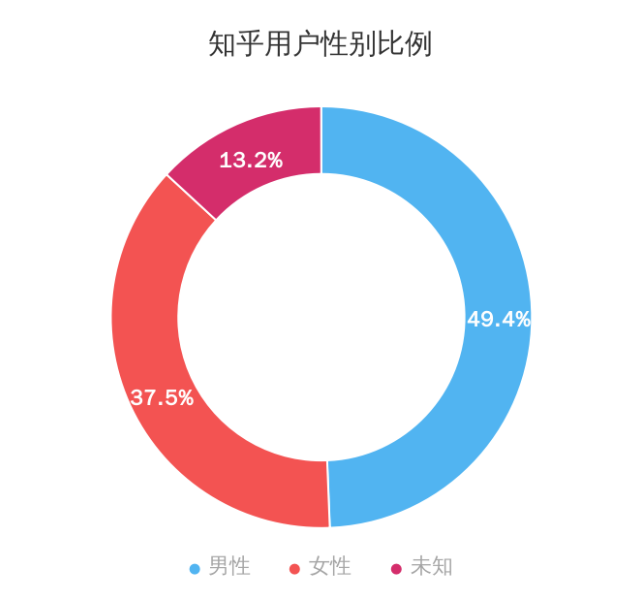
\includegraphics[width=\linewidth]{Wyonghu-3.png}
    \caption{性别比例}
  \end{subfigure}
  \begin{subfigure}[b]{0.49\linewidth}
    \centering
    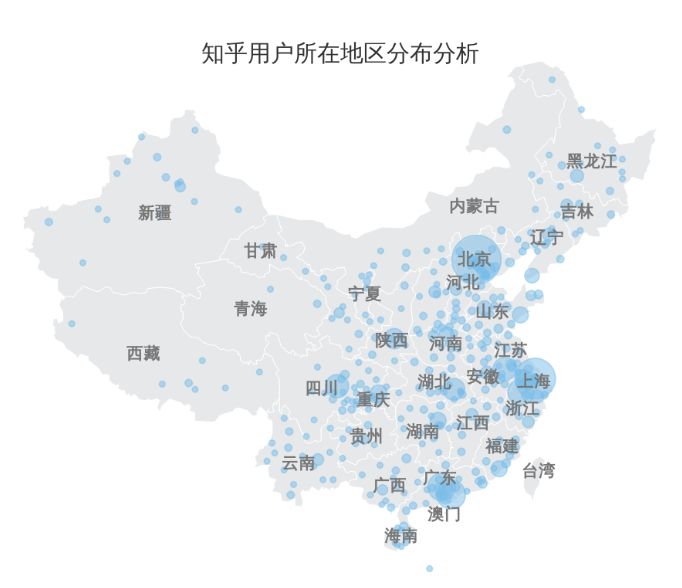
\includegraphics[width=\linewidth]{Wyonghu-2.png}
    \caption{N地区分布}
  \end{subfigure}
  \begin{subfigure}[b]{0.49\linewidth}
    \centering
    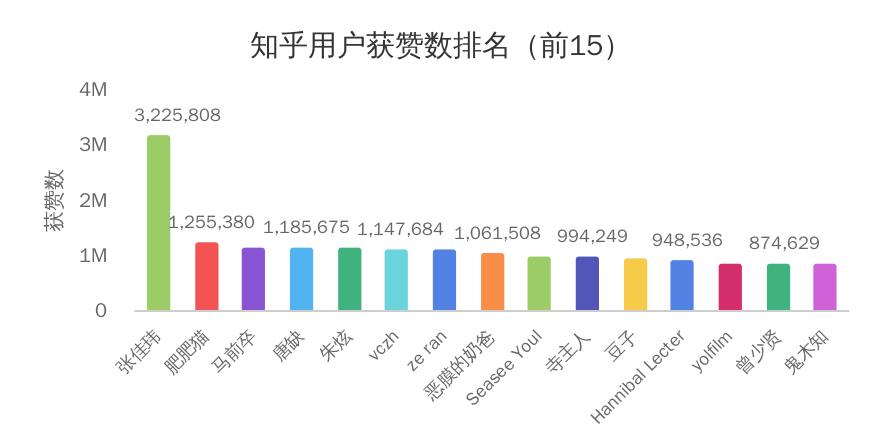
\includegraphics[width=\linewidth]{Wyonghu-4.png}
    \caption{赞数排名}
  \end{subfigure}
  \begin{subfigure}[b]{0.49\linewidth}
    \centering
    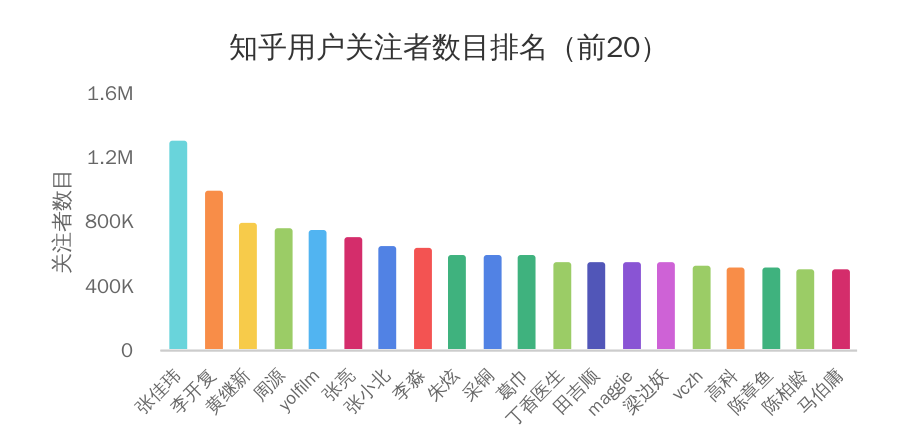
\includegraphics[width=\linewidth]{Wyonghu-6.png}
    \caption{关注数目排名}
  \end{subfigure}
  \caption{知乎用户数据可视化}
\end{figure}



% \chapter{聚类算法分析}
% 大数据不仅引起学术界和产业界的普遍重视,更上升为世界各国的国家战略.
% 然而,要充分发挥大数据的作用,必须具备强大的数据分析能力.
% 本章就无监督学习中的$K-means$算法进行研究,并分析算法的优缺点.
% 并将本章研究的算法运用到下一章节对具体数据进行聚类分析.

% \section{聚类算法}
% \subsection{简介}
% 什么是聚类呢?《周易·系辞上》说:“方以类聚,物以群分,吉凶生矣.”
% 聚类是把一个数据对象的集合划分成簇(子集),使簇内对象批次相似,
% 簇间对象不相似的过程,是大数据分析的基本工具.

% \subsection{聚类算法分类}
% 和分类(监督学习的主要任务)不同,
% 聚类是在无标记样本的条件下将数据分组,
% 从而发现数据的天然结构.聚类在数据分析中扮演重要的校色,
% 它通常被用于以下三个方面:

% (1)	发现数据的潜在结构:深入洞察数据、产生假设、检测异常、确定主要特征.

% (2)	对数据进行自然分组:确定不同组织之间的相似程度(系统关系).

% (3)	对数据进行压缩:将聚类原型作为组织和概括数据的方法.

% 这几个方面的功能是聚类既可以作为预处理程序,又可以作为独立的数据分析工具.

% 通过查阅文件和上网查找资料,总结了聚类的发展阶段如下图所示:

% \begin{figure}[h!]
%   \centering
%     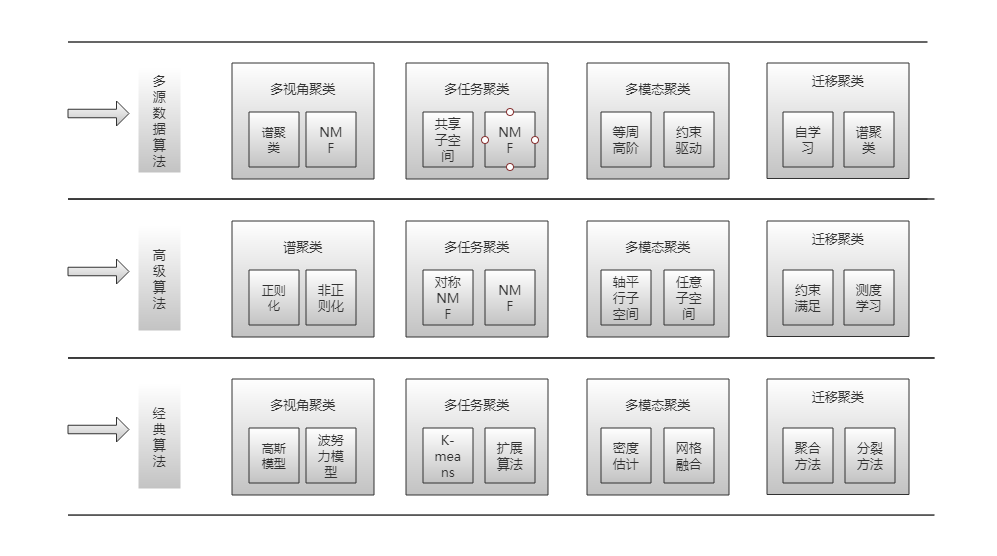
\includegraphics[width=1.0\linewidth]{Wjuleifazhan.png}
%   \caption{聚类发展}
% \end{figure}


% \section{$K-means$算法}
% \subsection{算法简介}
% $K-means$算法是由Steinhaus与1955年、
% Lloyd于1957年、Ball和Hall于1965年、
% Mcqueen于1967年分别在各自的不同的科学研究领域独立提出来的.
% 自被提出来以来,这一算法在许多学科领域得到了大量的研究和应用,
% 具体的例如数据压缩、数据分类、密度估计等诸多方面.
% 由于其算法思想简洁易懂,
% 而且对于许多聚类问题都可花费较小的计算代价而得到不错的聚类结果,
% $K-means$算法成为各种聚类算法中较为常用的算法之一,
% 至今仍然被广泛的使用,被学者们选为数据挖掘领域的十大算法之一.

% \subsection{算法思想}
% $K-means$算法继承了基于划分的聚类方法的基本思想.
% 基于划分的算法按某种目标将数据集划分成若干个组,
% 划分的结果就是使目标函数值最大化(或者最小化).
% 这样的优化目标通常是NP难的,因此采用某种贪心策略迭代求解.
% 具体的做法就是每个簇指定一个或者若干个代表点,
% 根据目标函数用这些代表点对这个数据集进行划分,
% 在划分结果中重新选择代表点,重复上述过程知道收敛.
% 贪心算法通常获得目标函数的局部最优解.
% 基于划分的算法基本上都以点对时间的聚类为标准,
% 而距离和簇代表点的选择至关重要.

% $K-means$算法在如何产生一个划分方面,
% $K-means$算法设定了每个划分的中心点,
% 从而形成以中心为分类依据的球星簇;
% 在验证所产生的划分是否合理方面,
% $K-means$算法以划分的类内紧致性作为标准,
% 具体来说,是以点与点之间的距离之和作为度量准则.
% 这种划分标准以及度量标准保证了算法可以很快达到收敛,
% 这就是$K-means$算法相比于其他算法的一个重大优势.

% \subsection{目标函数}
% 在K-menas算法中,
% 涉及计算每个对象与各个簇中心点之间的距离,
% 这个距离的度量也是用户自行设定的.
% 通常有闵可夫斯基、曼哈顿距离(L1范式)和欧几里得距离(L2)范式等.
% 针对不同的数据类型可以选取不同的距离度量标准.
% 在一般情况下,欧几里得是一个很好的度量数据间相似的标准,
% 也是大部分$K-means$算法中选定的距离度量标准.

% 聚类算法的目标通常用一个目标函数来表示.
% 采用欧几里得距离度量相似性的$K-means$算法,
% 使用误差的平方和(sum of squared errors,SSE)作为度量聚类质量的目标函数.
% 给定一个包含 $n$ 个数据对象的数据集合$D =\{ x_1, x_2, \cdots, x_n \}$,
% 定义经由$K-means$算法进行聚类分析后的产生的类别集合为$C=\{ C_1, C_2, \cdots, C_k \}$.
% 算法目标定义如下:
% \begin{equation}
%   \centering
%   SSE(C) = \sum_{ k=1}^{n} \sum_{x_i \in C_k} {\parallel x_i - c_k \parallel}^2 \qquad 
% \end{equation}
% 式中,$c_k$是簇$C_k$的中心点,计算方法如下所示:

% \begin{equation}
%   \centering
%   c_k = \frac {{\sum_{x_i \in C_k}^{n}} x_i} {\mid C_k \mid} \qquad
% \end{equation}

% $K-means$算法的目标就是能找到能最小化$SSE$的聚类结果,
% 这个最优化问题是一个NP难问题,
% 难以找到一个多项式算法对其求解.
% 不过可以将此问题进行转化,
% 通过不断迭代更新簇的构成和簇的中心点来进行最优化的求解,
% Lloyd算法就是此类算法.算法的迭代过程主要是:
% 第一步分配过程,在分配过程中,
% 每个数据样本都要被分配到离它距离最近的类中心所属的类中;
% 第二部更新过程,在更新过程中,类的中心点需要被重新计算
% ,采用分配到这一类别的所有样本数据对类中心点进行更新.
% Lloyd算法页被称为精确的$K-means$算法.

% 那么在簇中心 的更新过程中,为什么要选取均值作为计算标准呢?
% 为什么不是选择中位数等其他标准呢?
% 下面就从数学角度对这一问题做出详细的说明.
% 当邻近函数是欧几里得距离且目标是最小化SSE时,
% 选取均值点作为K-menas算法的簇中心点是可以从数学上推导出来的.
% 定义$C_k$为第$k$个簇,$x_i$是从属于$C_k$的数据点,
% $c_k$是$C_k$中所有数据 点的均值点.简化式(4-1),对于一维数组,
% 式可以写成

% \begin{equation}
%   \centering
%   SSE(C) = \sum_{k=1}^{k}\sum_{x \in C_k}\left(c_k-x_i\right)^2
% \end{equation}

% 为最小化$SSE$,对式(4-3)求导,令导数等于0,并求解$c_k$.其过程如下所示:

% \begin{equation}
%   \centering
%   \frac{\partial SSE}{\partial c_j} = 
%   \frac{\partial \sum_{k=1}^{k}\sum_{x \in C_k}\left(c_k-x_i\right)^2}
%   {\partial c_j} = \sum_{k=1}^{k}\sum_{x \in C_k} 
%   \frac{\partial \left(c_k-x_i\right)^2}{\partial c_j} = 
%   \sum_{x_i \in C_j} 2 \cdot \left(c_j - x_i\right) = 0
% \end{equation}

% \begin{equation}
%   \centering
%   \sum_{x_i \in C_j} 2 \cdot  \left( c_j - x_i \right) = 0 
%   \Rightarrow 
%   \vert C_j \vert \cdot c_j = \sum_{x_i \in C_j} x_i 
%   \Rightarrow 
%   c_j = \frac {\sum_{x_i \in C_j} x_i }{\vert C_j \vert}
% \end{equation}

% 经过以上的推导,最终得出的结果就是当导数为0时,
% 每个类中心的计算公式正好为计算该类中包含的所有数据点的均值公式,
% 因此,可以得出这样的结论:簇的最小化SSE的最佳中心点就是簇中各点的均值.


% \section{算法流程}
% \subsection{算法流程图}
% $K-means$算法采用了贪心算法,迭代的方式对聚类结果进行更新,
% 最终获得最小化的SSE.从某种某种角度上来说,$K-means$算法时EM算法的一种特例,
% 两者的思想都是先固定一个变量在对另一个变量进行更新,如此反复直到收敛为止.
% 算法流程如如下所示:

% \begin{figure}[h!]
%   \centering
%     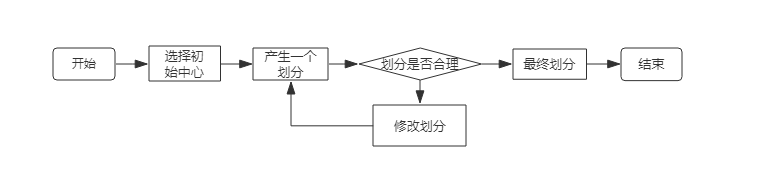
\includegraphics[width=1.0\linewidth]{Wsuanfaliuchengtu.png}
%   \caption{算法流程图}
% \end{figure}





% \subsection{算法步骤}

% $K-means$算法采用了贪心算法的思想,以迭代的方式对聚类结果进行更新,
% 最终获得最小的$SSE$.从某种角度来说,$K-means$算法是$EM$算法的一种特例,
% 两者的思想都是先固定一个变量然后在对另一个变量进行更新,如此反复直到收敛.
% 算法4.3给出了$K-means$算法的具体步骤: 

  

% \begin{algorithm}[htb]
%   \caption{ $K-means$}   
%   \label{alg:Framwork}   
%   \begin{algorithmic}[1] %这个1 表示每一行都显示数字  
%   \REQUIRE ~~\\ %算法的输入参数:Input  
%   All the set of point, $A$;\\  
%   The number of clusters, $k$.\\   
%   \ENSURE ~~\\ %算法的输出:Output  
%   $k$ cluster center points.\\
%   \STATE Randomly select k initial center points;    
%   \STATE  \textbf{repeat} 
%   \STATE \ \ \ \ Calculate the distance between each point and its own center point; \\
%   \STATE \ \ \ \ Assign the points to other clusters with the closest distance to your center;
%   \STATE \ \ \ \ By formula (4-5) obtained $c_k$, update the cluster center point;
%   \STATE  \textbf{until}  The center point does not change;
%   \RETURN $k$ coordinate. %算法的返回值  
%   \end{algorithmic}  
% \end{algorithm}  


% \section{算法实现与分析}
% \subsection{算法实现}
% 在$K-means$算法的实际执行过程中,
% 可能会出现已经进行了多次迭代而构成的簇还在发生变化的情况.
% 由于大部分的收敛都发生在早期阶段,在问题要求不是特别严格的情况下,
% 通常采用一种较弱的条件来替换算法的标准收敛条件,
% 例如“直到仅有1\%的点发生改变”,
% 这样弱化的收敛条件可以避免算法迭代次数过多的问题的发生,
% 在算法的精确性和时间效率上做出了一个平衡.算法执行构成如下图所示.

% \begin{figure}[h!]
%   \centering
%   \begin{subfigure}[b]{0.4\linewidth}
%     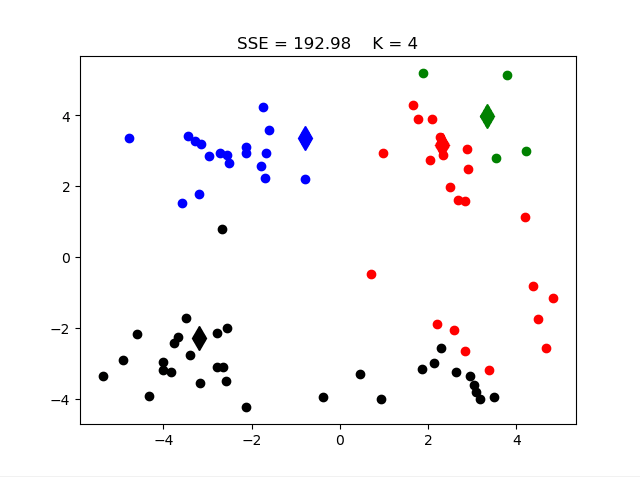
\includegraphics[width=\linewidth]{W4-1.png}
%     \caption{第一次迭代}
%   \end{subfigure}
%   \begin{subfigure}[b]{0.4\linewidth}
%     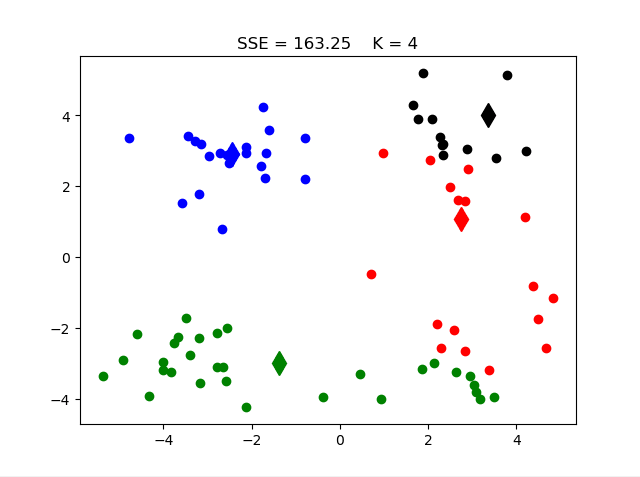
\includegraphics[width=\linewidth]{W4-2.png}
%     \caption{第二次迭代}
%   \end{subfigure}
%   \begin{subfigure}[b]{0.4\linewidth}
%     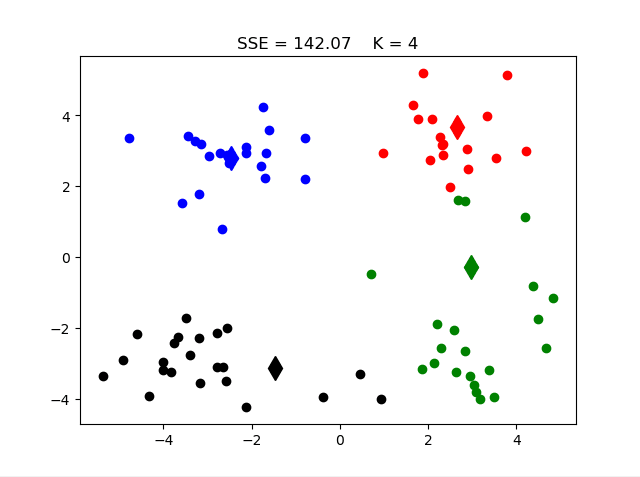
\includegraphics[width=\linewidth]{W4-3.png}
%     \caption{第三次迭代}
%   \end{subfigure}
%   \begin{subfigure}[b]{0.4\linewidth}
%     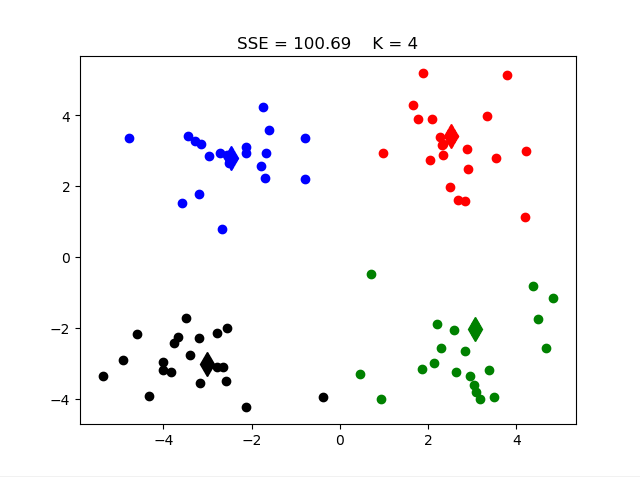
\includegraphics[width=\linewidth]{W4-4.png}
%     \caption{第四次迭代}
%   \end{subfigure}
%   \begin{subfigure}[b]{0.4\linewidth}
%     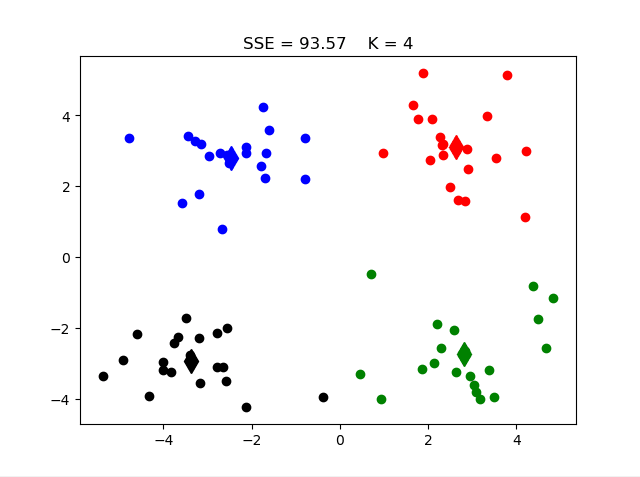
\includegraphics[width=\linewidth]{W4-5.png}
%     \caption{第五次迭代}
%   \end{subfigure}
%   \begin{subfigure}[b]{0.4\linewidth}
%     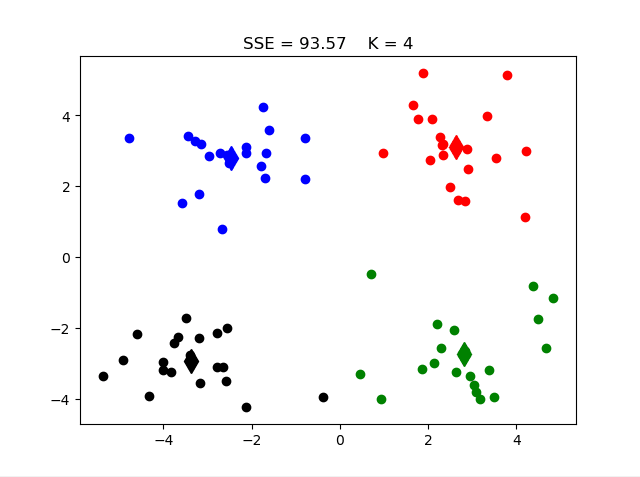
\includegraphics[width=\linewidth]{W4-6.png}
%     \caption{第六次迭代}
%   \end{subfigure}
%   \caption{$K-means$算法执行过程}
% \end{figure}

% 下面举例说明$K-means$算法是如何工作的.
% 如图4-3所示,数据集中一共包含四个类型的数据点,设定初始聚类个数为4.
% 首先,随机选取4个初始的中心点,即图中的钻石点.
% 接下来对于每个数据点,
% 计算它们与4个中心点的距离并选择最小的那个中心点,加入其表示的簇.
% 在是有数据点都分配完成后,计算每个簇中所有数据点的均值,
% 以此作为新的中心点,之后再次进行计算数据点与中心点之间的距离
% 来进行数据的重新分配,就形成了一次迭代后的数据分配.
% 重复进行分配和中心点更新这两个步骤,直至簇不在发生变化,
% 算法终止.如图4-3所示,(a)到(e)图中的中心点不点变化,
% 就是对中心点的不断更新,其中的有的数据点不断变化的颜色就是在进行重新分配,
% 直到(e)图,(e)图和(f)图是一样的,说明簇不在发生变化,算法终止.

% \subsection{性能分析}
% 下面对$K-means$算法的性能进行分析,主要是对算法的时间复杂度和空间复杂度进行分析.
% \begin{figure}[h!]
%   \centering
%   \begin{subfigure}[b]{0.8\linewidth}
%     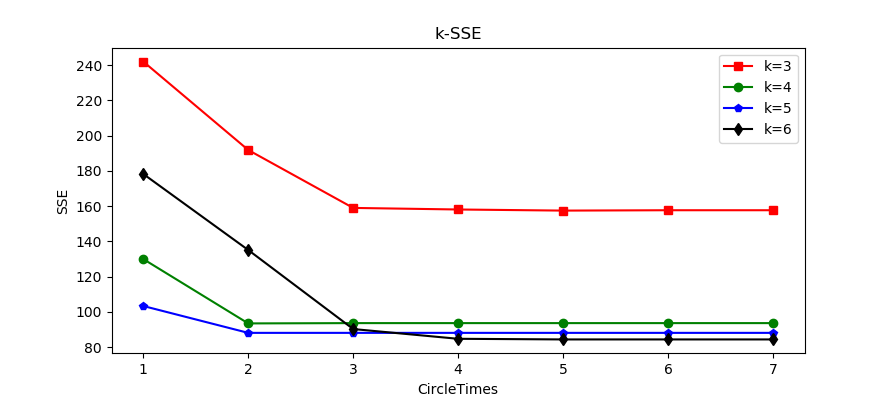
\includegraphics[width=\linewidth]{Wct-SSE-first.png}
%     \caption{实验1 k-SSE迭代图}
%   \end{subfigure}
%   \begin{subfigure}[b]{0.8\linewidth}
%     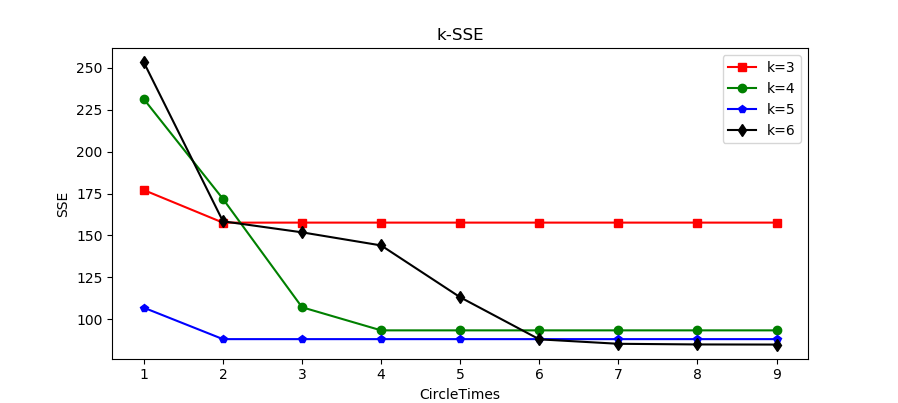
\includegraphics[width=\linewidth]{Wct-SSE-second.png}
%     \caption{实验2 k-SSE迭代图}
%   \end{subfigure}
%   \caption{性能分析}
% \end{figure}

% 在时间方面,$K-means$算法的时间需求基本上与数据点的个数成线性相关.
% 具体来说,其时间复杂度为$O(i*k*n*m)$,这里的$k$是簇的个数,
% $i$是迭代次数(CircleTimes),n是数据集中包含数据点的个数,
% m是每个数据的属性数.由于收敛大多发生在早期阶段,$i$的值通常比较小,
% 如上图所示,$i$为4就收敛了.这样,只要簇的个数$k$远小于$n$,
% 算法的计算时间就与$n$成线性相关.

% 在空间方面,$K-means$算法需要存放的类容只有数据点和每个簇的中心点数据.
% 具体来说,其空间复杂度为$O((k+n)*m)$,
% 这几个量的定义与计算时间复杂度时的定义一样.
% 一般可以认为,$i$,$k$和$m$都是常量.
% 这样的话,算法的时间复杂度和空间复杂度都可以简化为$O(n)$,即线性的.

% 由此可以看出,$K-means$是一种计算简单而又行至有效的聚类算法.

% 除了简单且有效以外,$K-means$算法还具有以下优点:

% (1)算法使用于各种数据;

% (2)当潜在的簇是凸的,
% 簇与簇之间大小相近且差异明显时,算法可以展现很好的聚类效果;

% (3)对于大规模数据集合,该算法非常高效且伸缩性较好

% 但是,$K-means$算法还存在一些不足之处:

% (1)首先,由于在中心点的更新步骤中,算法所使用的是簇内所包含的所有数据点的平均值.
% 如果在某一问题上无法定义簇内数据点的平均值,那么该算法无法发挥效果.
% 也就是说,该算法在处理具有分类属性的数据是就无从下手.

% (2)在算法的初始化过程中,簇个数$k$的值和初始中心点的选取都对算法结果有着巨大的影响,
% 不合适的初始化值设定很容易造成算法最终收敛到局部最优值,这使得算法对先于知识具有较强的依赖性.

% (3)算法对噪声点和离群点十分敏感,少量的异常数据就会对簇类平均值的计算造成巨大的干扰,
% 这种干扰很可能会造成簇划分不合理.

% 针对以上不足,我们可以从算法层面上对标准的$K-means$算法做出修改,
% 或是在初始化阶段完善对初始值的设定.
% 在接下来的的一节中,就改进初始化策略做出说明,提高了原有算法的性能,使算法具有更强的生命力.


% \subsection{初始的选择}
% 对于$K-means$算法,有几个十分重要的因素影响着算法的聚类效果,
% 其中包括簇数目的选定、初始中心点的选取、距离度量的选择以及收敛条件的设定.
% 距离度量和收敛条件在本节之前已经说明过,余下两项就是在算法的最初阶段决定的,
% 这两个部分的初始化会直接影响最终能否得到合适的簇.


% \begin{figure}[h!]
%   \centering
%   \begin{subfigure}[b]{0.4\linewidth}
%     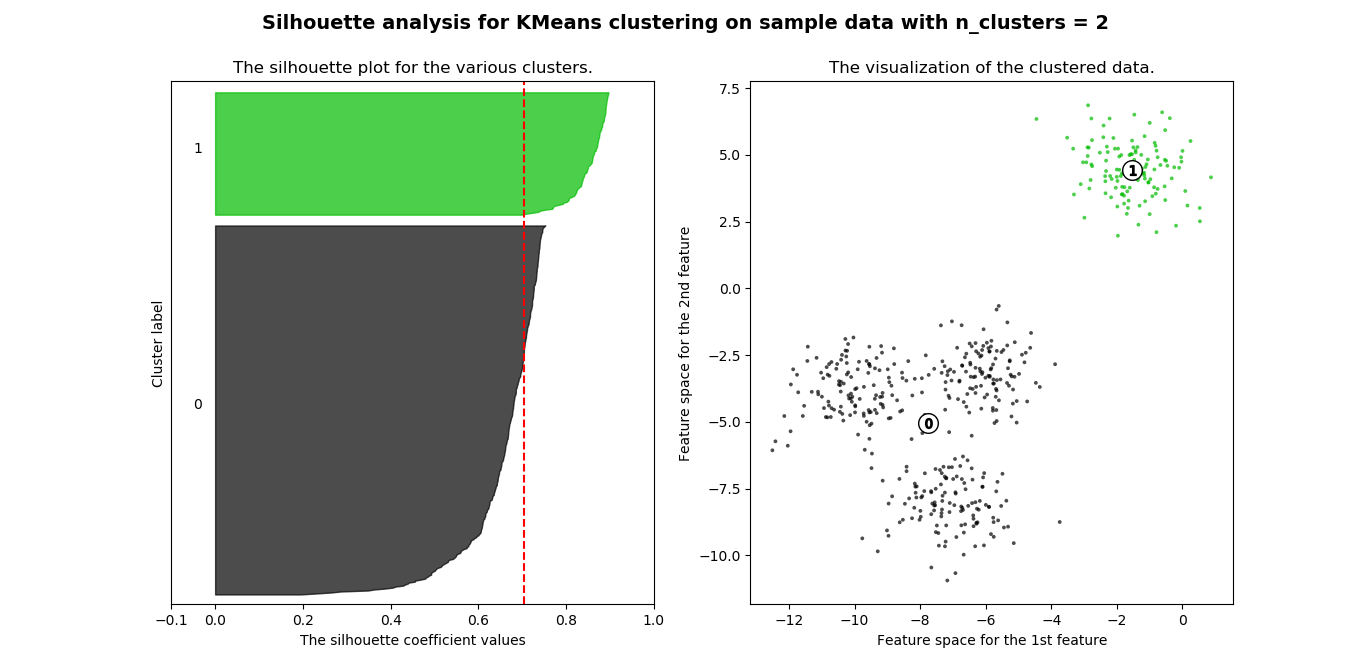
\includegraphics[width=\linewidth]{Wksh-2.png}
%     \caption{k=2}
%   \end{subfigure}
%   \begin{subfigure}[b]{0.4\linewidth}
%     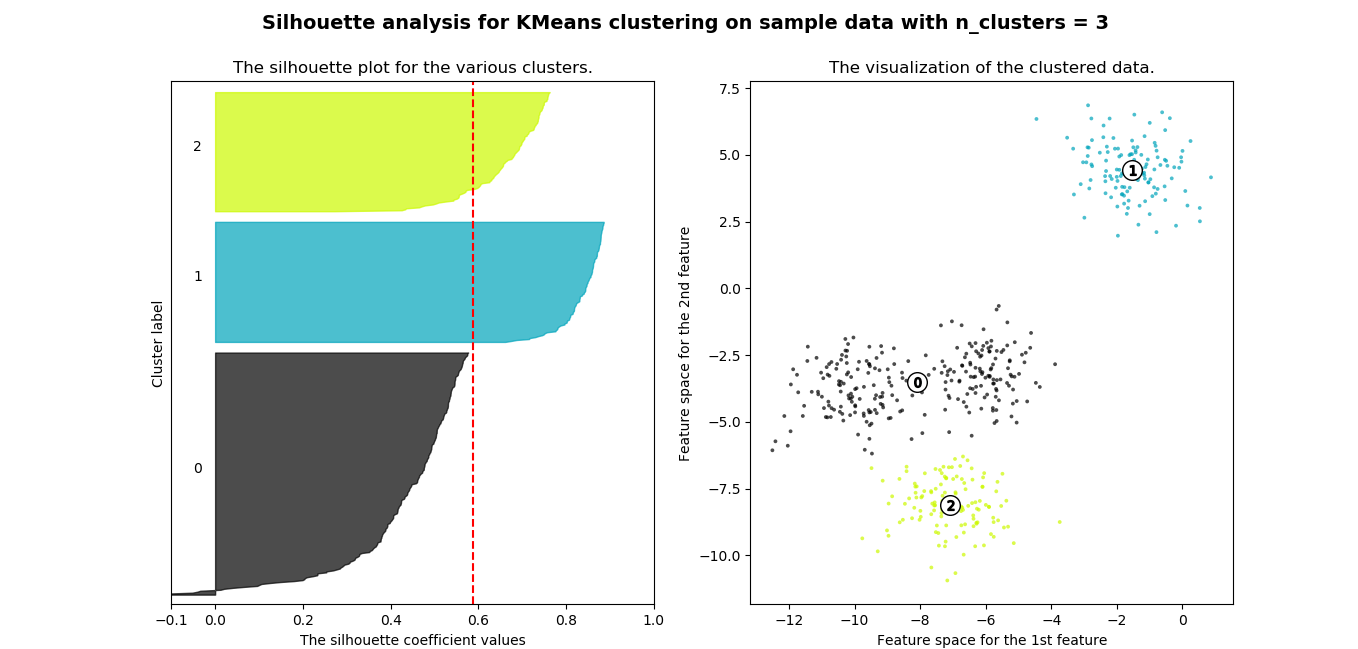
\includegraphics[width=\linewidth]{Wksh-3.png}
%     \caption{k=3}
%   \end{subfigure}
%   \begin{subfigure}[b]{0.4\linewidth}
%     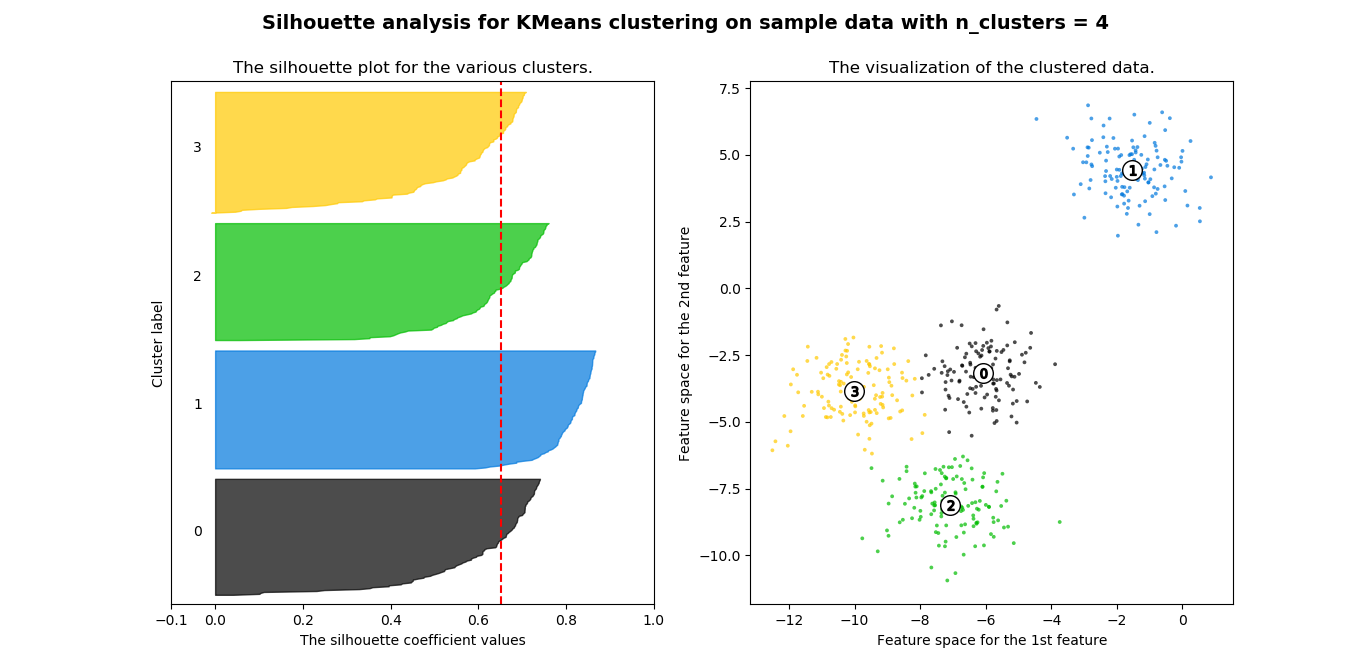
\includegraphics[width=\linewidth]{Wksh-4.png}
%     \caption{k=4}
%   \end{subfigure}
%   \begin{subfigure}[b]{0.4\linewidth}
%     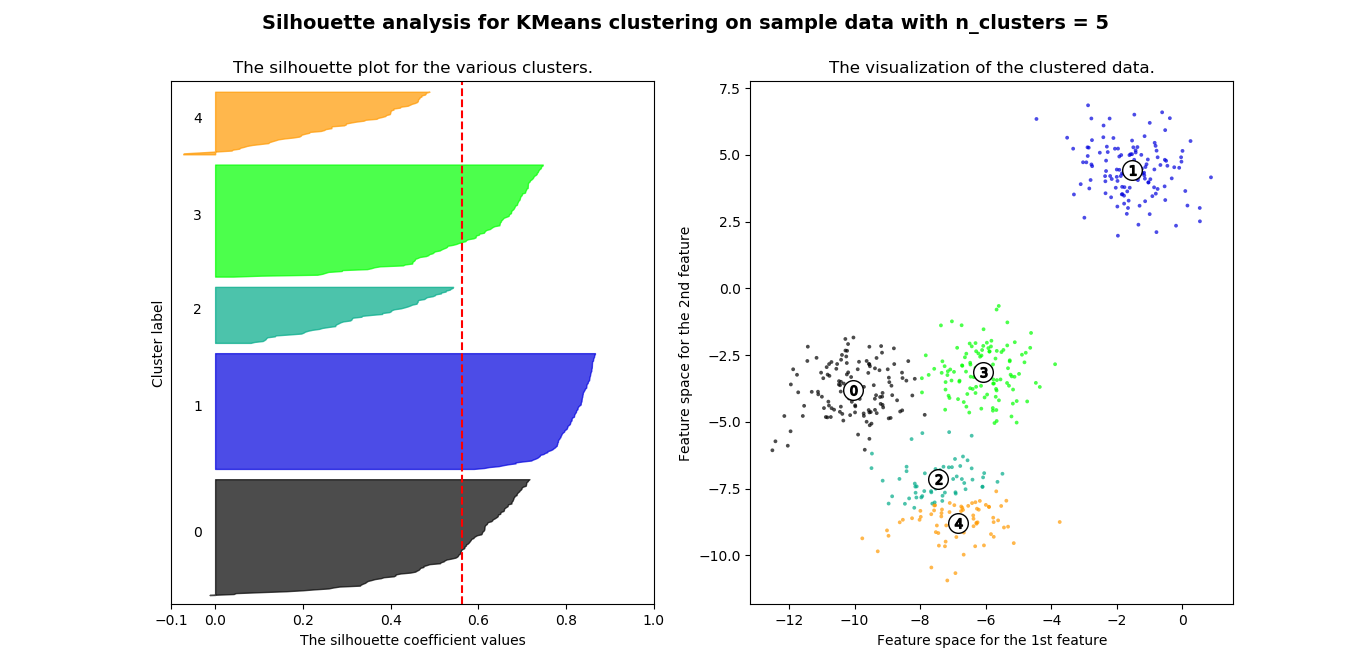
\includegraphics[width=\linewidth]{Wksh-5.png}
%     \caption{k=5}
%   \end{subfigure}
%   \begin{subfigure}[b]{1.0\linewidth}
%     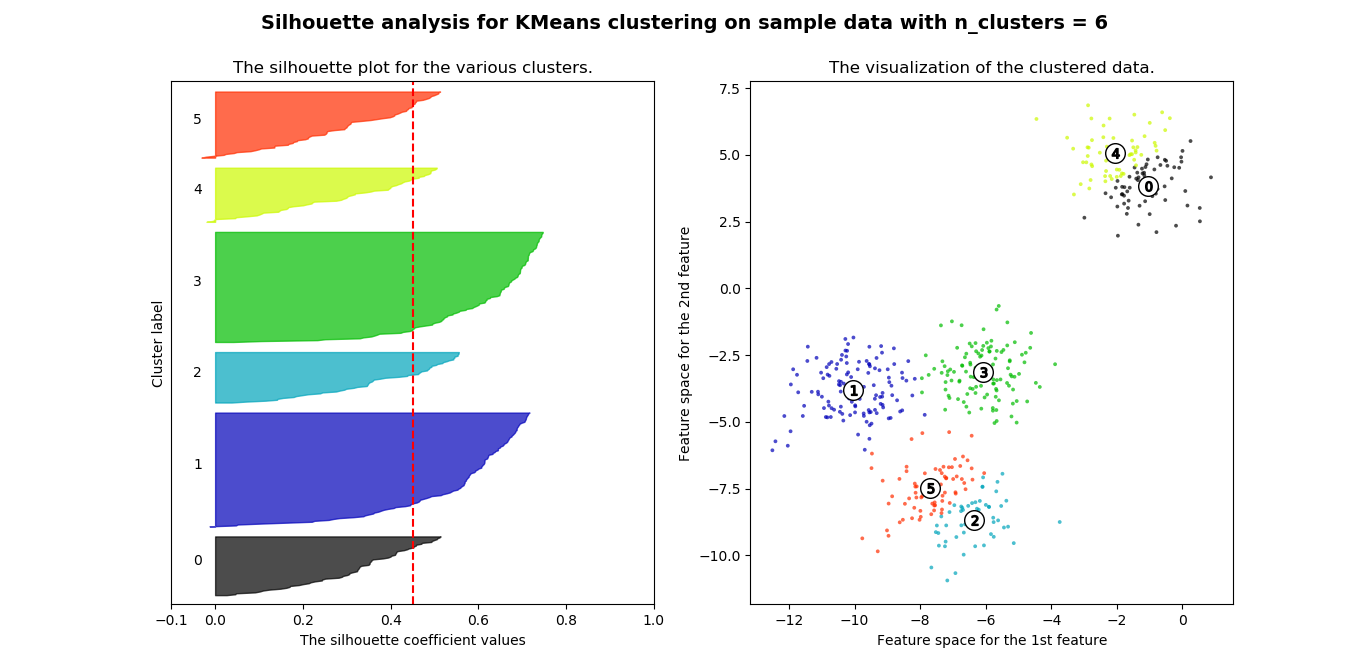
\includegraphics[width=\linewidth]{Wksh-6.png}
%     \caption{k=6}
%   \end{subfigure}
%   \caption{数据可视化}
% \end{figure}

% $K-means$聚类算法最被人诟病的是类别个数k的选择,
% 这个设定往往会对结果造成很大的影响,为此提出了一种可行的方法.
% 该方法是设定一个最大阈值,
% 令k从小到大逐渐增加,观察SSE的变化从而选取合适的k.
% 因为k-均值算法中的目标函数是距离的平方和,随着k的增大,
% 每个簇的类别相似性也随之增加,由此造成SSE的变化是单调的减小.
% 如果以算法目标为基准,选取使SSE最小的k,
% 则当k取最大值,即k为数据集中数据个数的时候对应SSE最小.
% 但这样做是毫无意义的,因为每个数据对对象单独成一个簇.
% 这种变化来确定SSE的方法中,需要绘制k-SSE折线图,如图4.4所示.
% 观察图像,在最初k很小的时候,k的增大会使SSE的值迅速减小,之后趋于平缓.
% 因此,选取图像中的拐点附近的值作为k的起始值,就可以得到很好的聚类效果.


% \begin{figure}[h!]
%   \centering
%     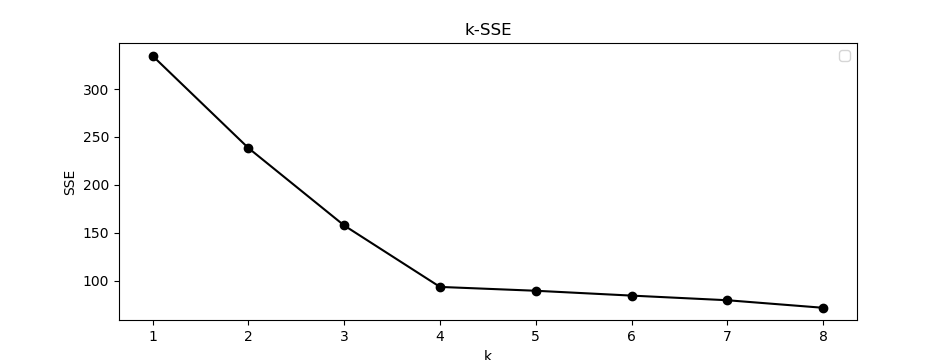
\includegraphics[width=0.8\linewidth]{Wk-SSE.png}
%   \caption{k-SSE折线图}
% \end{figure}



% 当然还有其他方法,如Calinski和Harabasz提出的Calinski-Harabasz指标、
% Tibshirani等提出的计算差异量统计值方法、
% 赤池信息准则(akaike information criterion,AIC)、
% 贝叶斯信息准则(Bayesian information criterion,BIC)、
% Newman和Girvan提出一种以结合层次聚类方法的k选取法、
% Ball和Hall提出一种迭代自组织的数据分析算法——ISODATA等方法.
% 本文就不介绍了,有兴趣的话可以查阅相关资料.

% 上文介绍的是k值的选取,
% 还有一个重要选择的就是初始点的选择.
% 最基本的初始点的选取方式就是随机选取k个点作为初始中心点,
% 这是Macqueen提出的方法.
% 然而这种方法很容易造成算法最终陷入一个局部最优的解,所得到的聚类分布并不是最优的.
% 针对这样的问题,
% 本文采用的一种有效的方法就是选取初始点是先从数据集中随机抽取一些子样本集,
% 对每一个子样本及都实施随机选取初始中心点的$K-means$算法.
% 将算法运行后产生的中心点放到一个集合当中,构成一个仅由中心构成的集合,
% 对这一集合进行聚类分析,将的带的结果作为原数据集的初始中心点.



% 当然不只这一中有效方法,还有两种方法,一种是将$K-means$算法与聚合层次聚类方法相结合,
% 另一种是采用最近邻密度的观点.本文对这两种方法也不做详细的介绍.


\chapter{知乎用户的复杂网络研究}
本章节主要对知乎用户信息资料进行分析,通过采用聚类算法和复杂网络技术对数据之间的关系进行分析,
得出数据实体的关系聚类图,分析算法的实际效果.
\section{知乎用户资料的特征分析}
对知乎用户资料的分析,为了判断该用户的重要程度,首先对用户的关注数、粉丝数(关注者数)、回答数、赞同数、感激数的的
平均数、中位数以及标准差进行了简单的统计,一共统计知乎用户数量153913,
统计结果如下所示:


\begin{figure}[h!]
  \centering
  \begin{subfigure}[b]{0.49\linewidth}
    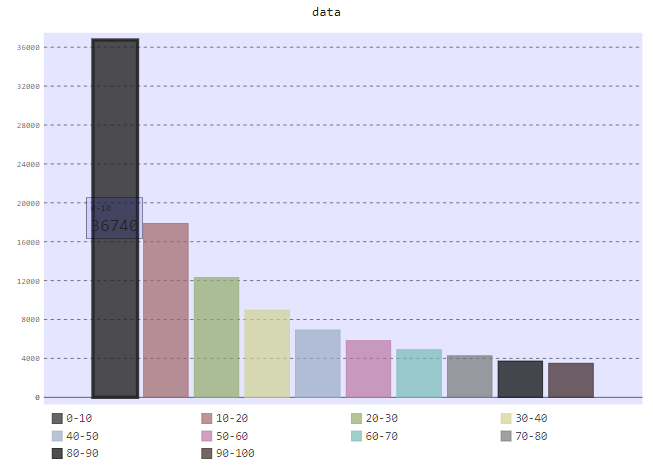
\includegraphics[width=\linewidth]{Wtongji-1.png}
    \caption{关注数100以内的统计结果}
  \end{subfigure}
  \begin{subfigure}[b]{0.49\linewidth}
    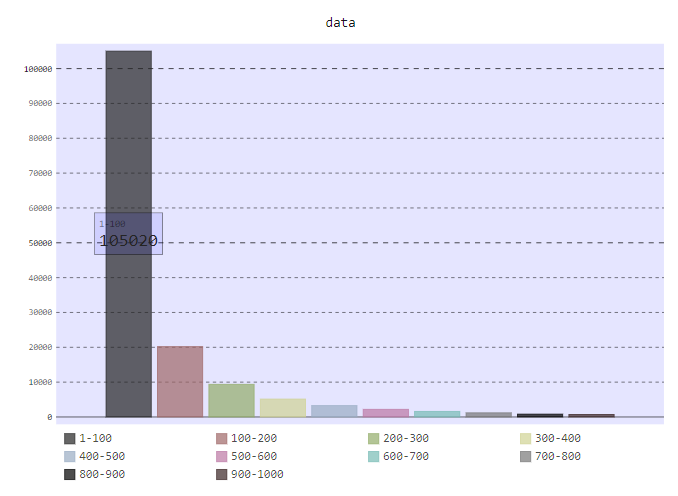
\includegraphics[width=\linewidth]{Wtongji-2.png}
    \caption{所有统计结果}
  \end{subfigure}
  \caption{following统计结果}
\end{figure}

\begin{table}[ht]
  \centering
  \begin{tabular}{p{0.15\textwidth}<{\centering}p{0.15\textwidth}<{\centering}p{0.1\textwidth}<{\centering}p{0.15\textwidth}<{\centering}}
    \toprule
    \textbf{type } & \textbf{ mean } & \textbf{ median} & \textbf{ Std }\\
    \midrule
    \textbf{following}   &  167.9845     &   42   &   470.62  \\
    \textbf{follower}    &  1277.1270    &   9    &   14022.77\\
    \textbf{answer}      &  38.2021      &   3    &   187.93 \\
    \textbf{voteup}      &  2992.0210    &   3    &   27399.50  \\
    \textbf{thanked}     &  513.0559     &   1    &   4438.83\\
    \bottomrule
  \end{tabular}
  \caption{统计结果}
\end{table}


在知乎用户之间一共存在三种关系,一种是用户甲关注用户乙,此时甲可以收到乙回答问题的信息推送和乙的动态,
第二种关系是用户甲被用户乙,此时乙就变成甲的粉丝
第三种是用户甲和用户乙相互关注,两人就变成了简单的好友关系,可以相互收到对方的信息.
根据图论知识我们可以简单知道,可以把用户当作节点,
用户之间的关系可以简化为无权有向图. 

要对知乎用户信息进行复杂网络特征分析,就自然而然的想得到了第二章所介绍到的聚类系数和度分布,
下图是知乎用户的入度和出度分布:

\begin{figure}[h!]
  \centering
  \begin{subfigure}[b]{0.49\linewidth}
    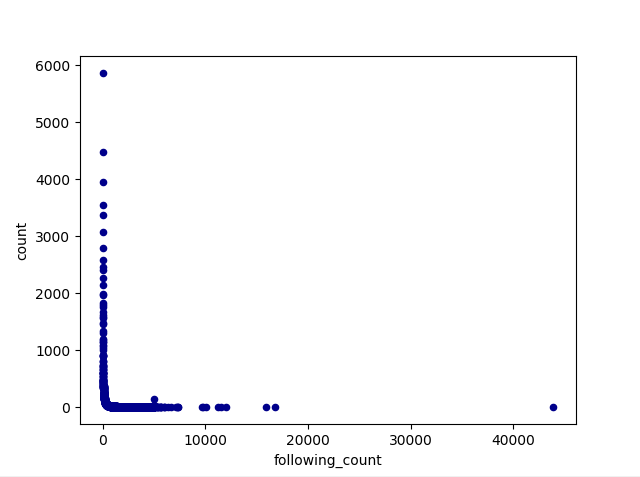
\includegraphics[width=\linewidth]{Wfollowing-1.png}
    \caption{}
  \end{subfigure}
  \begin{subfigure}[b]{0.49\linewidth}
    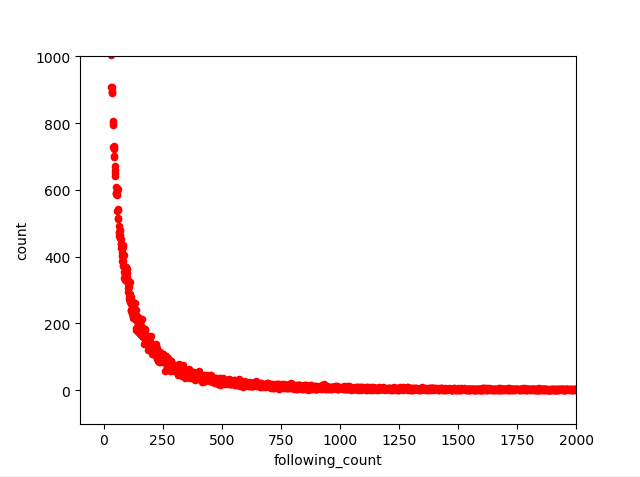
\includegraphics[width=\linewidth]{Wfollowing-2.png}
    \caption{}
  \end{subfigure}
  \caption{知乎用户出度分布}
\end{figure}



\begin{figure}[h!]
  \centering
  \begin{subfigure}[b]{0.49\linewidth}
    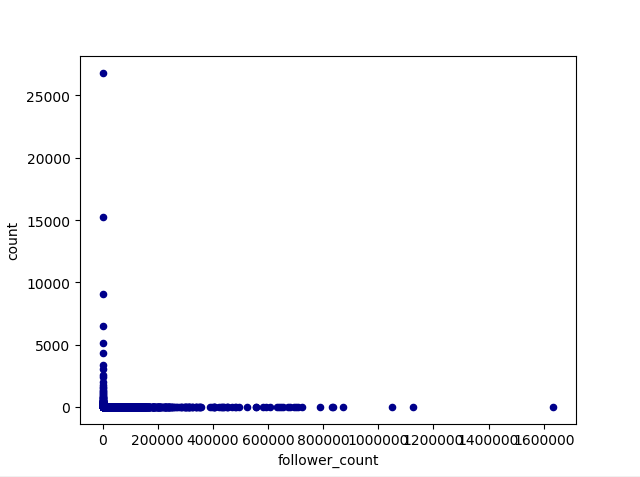
\includegraphics[width=\linewidth]{Wfollower-1.png}
    \caption{}
  \end{subfigure}
  \begin{subfigure}[b]{0.49\linewidth}
    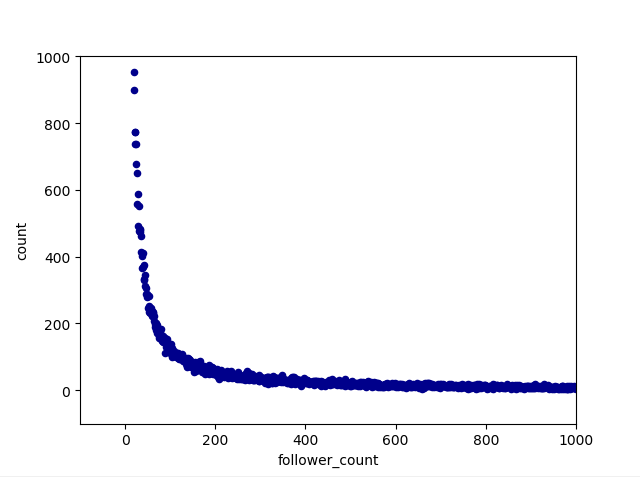
\includegraphics[width=\linewidth]{Wfollower-2.png}
    \caption{}
  \end{subfigure}
  \caption{知乎用户入度分布}
\end{figure}


由于图5-1(a)用户数量太多,用户之间的差距太大,所以用户之间的关系不是很明显,
因此把坐标的范围缩小到合适的大小后得到了5-1(b)的图像,入度分布处理和出度分布处理一样.

根据图的分布我们很自然的想到了幂律分布,
为了进一步得到明显的拟合曲线我们将幂律公式做以下处理:

根据幂律分布公式:

\begin{equation}
  y = cx^{-r}
\end{equation}

对式子两边同时取对数,可以得到:
\begin{equation}
  lny = lnc -rlnx
\end{equation}

在令两个$lny$和$lnx$分别为两个变量,在图形上很明显就可以看出变量是否符合幂律分布模型.

\begin{figure}[h!]
  \centering
  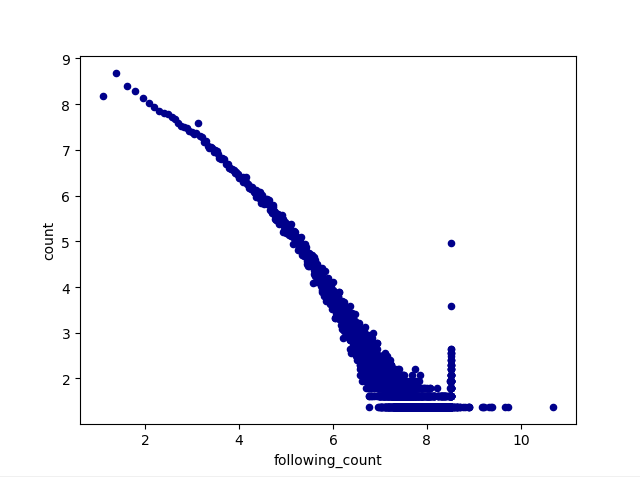
\includegraphics[width=0.8\linewidth]{Wlog.png}
  \caption{取对数度分布}
\end{figure}

由此就可以轻易地看出,知乎用户网络的度分布符合幂律分布.
现在我们需要对数据进行线性回归分析,本文用到的工具是python的Statsmodels统计包.
本文重点介绍回归信息中最常用的OLS(ordinary least square)功能.

\begin{figure}[h!]
  \centering
  \includegraphics[width=0.8\linewidth]{Wnihe.png}
  \caption{拟合曲线}
\end{figure}

针对知乎用户的出度分布,采用OLS方法对数据进行拟合得到结果如下表所示:
\begin{figure}[h!]
  \centering
  \includegraphics[width=0.8\linewidth]{Wnihejieguo.png}
  \caption{拟合效果分析}
\end{figure}

由表我们可以得到拟合曲线为$lny$ = 8.804\ -\ 2.7128$lnx$,
由此可以得到拟合的幂律公式为$y = 6660.83 \times x^{-2.7128}$,
拟合效果(R-squared:)为0.982.

可以从图中看出,虽然统计时出度为0的数目为3541,
其中不乏有大量的僵尸粉对拟合效果造成了一定的影响,
但是总体上知乎用户关系之间的网络还是具有复杂网络具有的特征,
符合BA无标度网络模型.



\section{K-means算法}
\subsection{算法介绍}
K-means是典型的基于划分思想的聚类.
那么什么是聚类呢?《周易·系辞上》说:“方以类聚,物以群分,吉凶生矣.”
聚类就是是把数据对象的集合划分成不同簇,使簇内对象批次相似,
簇间对象不相似的过程,是大数据分析的基本工具.

通过查阅文件和上网查找资料,总结了聚类的发展阶段如下图所示:

\begin{figure}[h!]
  \centering
    \includegraphics[width=1.0\linewidth]{Wjuleifazhan.png}
  \caption{聚类发展}
\end{figure}


\subsection{算法思想和算法流程}
K-meas的算法\cite{张建萍2007基于聚类分析的}思想是基于划分的聚类方法,
将数据集按照算法进行划分若干组,采用贪心迭代求解.
具体做法如下:先选定分成的多少簇,根据目标函数对数据集进行划分,
不满足目标函数时,继续重新选择代表点重复上述构成直到收敛.

目标函数通常选择点和点之间的距离之和作为度量准则,
这种方法可以保证算法以更快的速度达到收敛.距离我们采用的欧几里得距离(L2)范式.
对数据集合$D =\{ x_1, x_2, \cdots, x_n \}$,进算法进行划分后集合为$C=\{ C_1, C_2, \cdots, C_k \}$.
目标函数计算如下
\begin{equation}
  \centering
  SSE(C) = \sum_{ k=1}^{n} \sum_{x_i \in C_k} {\parallel x_i - c_k \parallel}^2 \qquad 
\end{equation}
式中,$c_k$是簇$C_k$的中心点,计算方法如下所示:
\begin{equation}
  \centering
  c_k = \frac {{\sum_{x_i \in C_k}^{n}} x_i} {\mid C_k \mid} \qquad
\end{equation}

算法目标就是通过不断的迭代选择能够最小化SSE的聚类结果.
选择均值作为SSE的最好中心点的原因如下推导:
\begin{equation}
  \centering
  SSE(C) = \sum_{k=1}^{k}\sum_{x \in C_k}\left(c_k-x_i\right)^2
\end{equation}

对式求导,令导数等于0.

\begin{equation}
  \centering
  \frac{\partial SSE}{\partial c_j} = 
  \frac{\partial \sum_{k=1}^{k}\sum_{x \in C_k}\left(c_k-x_i\right)^2}
  {\partial c_j} = \sum_{k=1}^{k}\sum_{x \in C_k} 
  \frac{\partial \left(c_k-x_i\right)^2}{\partial c_j} = 
  \sum_{x_i \in C_j} 2 \cdot \left(c_j - x_i\right) = 0
\end{equation}

\begin{equation}
  \centering
  \sum_{x_i \in C_j} 2 \cdot  \left( c_j - x_i \right) = 0 
  \Rightarrow 
  \vert C_j \vert \cdot c_j = \sum_{x_i \in C_j} x_i 
  \Rightarrow 
  c_j = \frac {\sum_{x_i \in C_j} x_i }{\vert C_j \vert}
\end{equation}
式子中$C_k$为第$k$个簇,$x_i$是从属于$C_k$的数据点,$c_k$是$C_k$中所有数据点的均值点.

算法流程图如下:
\begin{figure}[h!]
  \centering
    \includegraphics[width=1.0\linewidth]{Wsuanfaliuchengtu.png}
  \caption{算法流程图}
\end{figure}

算法步骤:
\begin{algorithm}[htb]
  \caption{ $K-means$}   
  \label{alg:Framwork}   
  \begin{algorithmic}[1] %这个1 表示每一行都显示数字  
  \REQUIRE ~~\\ %算法的输入参数:Input  
  All the set of point, $A$;\\  
  The number of clusters, $k$.\\   
  \ENSURE ~~\\ %算法的输出:Output  
  $k$ cluster center points.\\
  \STATE Randomly select k initial center points;    
  \STATE  \textbf{repeat} 
  \STATE \ \ \ \ Calculate the distance between each point and its own center point; \\
  \STATE \ \ \ \ Assign the points to other clusters with the closest distance to your center;
  \STATE \ \ \ \ By formula (4-5) obtained $c_k$, update the cluster center point;
  \STATE  \textbf{until}  The center point does not change;
  \RETURN $k$ coordinate. %算法的返回值  
  \end{algorithmic}  
\end{algorithm}  

\subsection{性能分析}
为了更好的分析算法性能,现在对一组数据进行迭代分析,迭代过程如下图所示:

\begin{figure}[h!]
  \centering
  \begin{subfigure}[b]{0.4\linewidth}
    \includegraphics[width=\linewidth]{W4-1.png}
    \caption{第一次迭代}
  \end{subfigure}
  \begin{subfigure}[b]{0.4\linewidth}
    \includegraphics[width=\linewidth]{W4-2.png}
    \caption{第二次迭代}
  \end{subfigure}
  \begin{subfigure}[b]{0.4\linewidth}
    \includegraphics[width=\linewidth]{W4-3.png}
    \caption{第三次迭代}
  \end{subfigure}
  \begin{subfigure}[b]{0.4\linewidth}
    \includegraphics[width=\linewidth]{W4-4.png}
    \caption{第四次迭代}
  \end{subfigure}
  % \begin{subfigure}[b]{0.4\linewidth}
  %   \includegraphics[width=\linewidth]{W4-5.png}
  %   \caption{第五次迭代}
  % \end{subfigure}
  % \begin{subfigure}[b]{0.4\linewidth}
  %   \includegraphics[width=\linewidth]{W4-6.png}
  %   \caption{第六次迭代}
  % \end{subfigure}
  \caption{$K-means$算法执行过程}
\end{figure}

下面对算法的时间复杂度和空间复杂度进行分析:

时间复杂度:$K-means$算法的时间需求大体上与数据点的个数成线性相关.
具体来说,其时间复杂度为$O(i*k*n*m)$,$k$是簇的个数,
$i$是迭代次数,n是数据集中数据点的个数,
m是每个数据的属性数.由于收敛大多发生在早期阶段,$i$的值通常比较小,
如上图所示,$i$为4就收敛了.这样,只要簇的个数$k$远小于$n$,
算法的计算时间就与$n$成线性相关.

空间复杂度:$K-means$算法需要存放的类容只有数据点和每个簇的中心点数据.
具体来说,其空间复杂度为$O((k+n)*m)$,
这几个量的定义与计算时间复杂度时的定义一样.
一般可以认为,$i$,$k$和$m$都是常量.
这样的话,算法的时间复杂度和空间复杂度都可以简化为$O(n)$,也是线性的.

故可以看出该算法是一种计算简单而有效的聚类算法.

\begin{figure}[h!]
  \centering
  \begin{subfigure}[b]{0.8\linewidth}
    \includegraphics[width=\linewidth]{Wct-SSE-first.png}
    \caption{实验1 k-SSE迭代图}
  \end{subfigure}
  \begin{subfigure}[b]{0.8\linewidth}
    \includegraphics[width=\linewidth]{Wct-SSE-second.png}
    \caption{实验2 k-SSE迭代图}
  \end{subfigure}
  \caption{性能分析}
\end{figure}

\section{实验过程}
\subsection{实验环境}
本章节主要使用的开发软件是Gephi,Gephi继承了图论中对图的定义,
也使用了相同的概念和术语,也有部分相同的研究内容,且包含了网络科学中对网络研究的模式和方法.
Gephi是在Netbeans平台上开发,语言是JAVA,并且使用OpenGL作为它的可视化引擎.
本文实验环境如下表所示:
\begin{table}[h!]
  \centering\begin{tabular}{cccc}
    \toprule
    \textbf{类别} & \textbf{描述} & \textbf{类别}  & \textbf{描述}\\
    \midrule
    开发语言  &  Python3.6                &  开发软件  &  Gephi0.92 \\
    操作系统  &  Windows10 pro            &  系统环境  &  Anaconda4.5 \\
    CPU型号   &  Intel i5-4210M           &  内存大小  & 4GB \\
    GPU型号   & Intel(R)HD Graphics 4600  &  显存大小  & 2GB \\   
    \bottomrule
  \end{tabular}
  \caption{实验环境}
\end{table}

\subsection{实验结果}
用户关注的人可以体现出用户的兴趣所在,对用户的出度进行聚类分析,
聚成的类即表示用户的兴趣,取采集数据的前一千数据进行分析.
由于K-means的聚类方法中的聚类个数不能确定,
为了防止实验误差,做了两次实验:
\begin{figure}[h!]
  \centering
  \begin{subfigure}[b]{0.49\linewidth}
    \includegraphics[width=\linewidth]{diedaigoucheng.png}
    \caption{K-means实验过程}
  \end{subfigure}
  \begin{subfigure}[b]{0.49\linewidth}
    \includegraphics[width=\linewidth]{Kzhiduibi.png}
    \caption{K-meansK的K值选择}
  \end{subfigure}
  \caption{聚类分析}
\end{figure}

对图中的函数关系可以看出,随着K值的增大,SSE越来越小,说明聚类个数越多聚类效果越好(SSE越小)
,但是为了选取使SSE最小的K值,那么就是说K取最大值即每个数据为一个类,显然这样做是毫无意义的.
因此我们应该采取适当的方法来确定合适的K值,从图像中可以看出,当K很小时,SSE很大,
随着K的增大SSE迅速减小.所以我们可以选取趋于平缓的K值作为聚类结果即可,
这里的K可以取大于12的值,都可以取得很好的聚类效果.
选取K值为15时的聚类结果如下图所示:
\begin{figure}[h!]
  \centering
    \includegraphics[width=1.0\linewidth]{juleijiegou.png}
  \caption{聚类结果}
\end{figure}

\subsection{实验改进}
从上一节的聚类结果来看,聚类结果并不是很显著,因此对实验进行改进.

算法采用的是复杂网络中的社团发现算法,同K-means聚类算法一样,不能事先确认社区的数目,
于是必须有一种度量的方法,本文采用的是模块度的度量方法进行的实验.
用模块度来衡量社区的划分是不是相对比较好的结果.好的聚类结果在社区内部的节点相似度比较高,
而在社区外部节点的相似度较低.通常来说,当模块度值越大说明网络的划分比较理想,
模块度值范围一般在0到1之间,值越大则可以说明社区结构准确度越高,在实际网络中,比较理想的模块度的值一般介于0.3
到0.7之间.

现在对第三章爬取的数据为数据集,选取11109个实验节点,边13487条,
实验结果如下:

\begin{figure}[h!]
  \centering
  \begin{subfigure}[b]{0.4\linewidth}
    \includegraphics[width=\linewidth]{Gephi1.png}
    \caption{}
  \end{subfigure}
  \begin{subfigure}[b]{0.4\linewidth}
    \includegraphics[width=\linewidth]{Gephi5.png}
    \caption{}
  \end{subfigure}
  \begin{subfigure}[b]{0.4\linewidth}
    \includegraphics[width=\linewidth]{Open1.png}
    \caption{}
  \end{subfigure}
  \begin{subfigure}[b]{0.4\linewidth}
    \includegraphics[width=\linewidth]{Open2.png}
    \caption{}
  \end{subfigure}
  \caption{实验结果}
\end{figure}
实验结果分析:
聚类结果一共形成了24类,并以不同的颜色表示出来,
其中用户vczh和Stuff共同关注27个人,这些人大都喜欢摄影和旅游,
然后通过他们的主页观察他们的赞助的Live,关注的话题,关注的专栏,
可以验证分析他们的兴趣确实有摄影和旅行.实验取得了良好的聚类效果.
网络特征如下:
\begin{table}[ht]
  \centering\begin{tabular}{cccc}
    \toprule
    \textbf{网络特征} & \textbf{参数} &   \textbf{网络特征} & \textbf{参数}\\
    \midrule
    平均度  &  1.214  &   模块度  &  0.738 \\
    平均加权度  &  1.223  & 网络直径  &  6     \\
    平均聚类系数    &  0.028 & 平均路径长度 &  2.85 \\
    \bottomrule
  \end{tabular}
  \caption{实验结果}
\end{table}

从数据结果来看,模块度的值为0.738,大于0.3说明聚类结构还是比较理想的.





% \subsection{实验结果与分析}
% 通过上文得知 知乎用户网络关系具有复杂网络的特征,那么复杂网络另一个重要的性质就是聚类系数.
% 就用第二章中的知识对用户之间的聚类系数进行计算:

% $$ C = \frac{3 \times \text{三角形的总数}}{\text{网络中三个连通节点的总数}} = 0.2698$$.


\section{小结}
通过实验可以看出K-means算法的优点:
算法可以使用于各种数据;当数据的簇是凸的,
簇与簇之间大小相近且差异明显时,算法可以表现出良好的聚类效果;
对于大规模数据集合,该算法非常高效且伸缩性较好.

本章节对用户之间的网络关系进行分析,通过复杂网络技术对用户进行聚类,得出用户的实体聚类图,
取得了良好的效果,得出了知乎用户关系复合复杂网络中的WS小世界模型,具有复杂网络的特性,
并计算出了复杂网络的特征.K-means算法还存在一些不足,该算法在处理具有分类属性的数据就无从下手,
初始值的选取对算法比较重要,算法对噪声点和离群点比较敏感等缺点.








\chapter{结论与展望}
本文主要对基于复杂网络的知乎用户数据挖掘惊醒总结,阐述本论文的主要成果和优点,
并总结论文中的方法还存在改进和完善的地方.

\section{结论}

数据挖掘可以通过预测未来的趋势,做出前瞻性的,具有理论依据的决策具有重要意义.
从大量信息中发现隐含的,有价值的信息是数据挖掘的目标,而聚类是数据挖掘中的重要一环.
本文数据挖掘的主要任务是对数据进行采集,并基于复杂网络技术对用户之间的关系进行分析,
得出用户实体聚类图,取得了不错的效果

总结来说,本文的主要成果如下:

(1)对复杂网络技术和知识以及复杂网络特征进行简单的分析,通过研究文献对相关研究做出了一定的综述工作.

(2)针对特定的挖掘数据进行大量的采集,并对用户数据进行简单的可视化工作.

(3) 针对本文采用的聚类算法进行充分的研究,研究算法的优势和缺点,并对算法进行了适当的改进.

(4) 通过对知乎用户之间的网络进行分析,得出用户之间的网络具有复杂网络的特征,
同时采用复杂网络技术对知乎用户之间进行分析,计算用户之间的相异度,
得出用户之间的实体聚类图并分析实际效果

\section{不足与展望}
因为数据挖掘本身就是一件复杂的研究领域,所以由于条件和时间等方面的原因,
本文的方法还存在需要改进和完善的地方,主要如下:

(1)爬取用户资料没有使用知乎API,而是采用的Scrapy框架,
爬取效果并不是很好,速度有点慢.
以后再进行大数据爬取是可以采用API爬取或者使用分布式,可以大大提高采集速度.

(2)在对知乎用户资料分析时,采用的算法在时间和空间开销存在着很大的优化空间,
而且在针对大量的数据时,会消耗大量的资源和时间,一部分原因可能存在电脑配置不够高的结果.
在未来的研究生涯中,可以针对优化算法的时间复杂度和资源优化可以进一步改善.

(3)在分析知乎用户之间的复杂网络的关系,只能对用户之间的关系进行简单的分析,
下一步工作对用户的行为进行分析,采集大量的用户行为信息(比如用户的回答,发布的文章,评论等)
这些都可以体现用户的兴趣所在,因此在未来的研究中,可以对文本信息进行文本划分以及文本分类,
进而构建用户兴趣建模,更加深度的对用户进行分析.



% 参考文献.应放在\backmatter之前.
% 推荐使用BibTeX,若不使用BibTeX时注释掉下面一句.
\nocite{*}
\bibliography{bachelor}
% 不使用 BibTeX
%\begin{thebibliography}{2}
%
%\bibitem{deng:01a}
%{邓建松,彭冉冉,陈长松}.
%\newblock {\em \LaTeXe{}科技排版指南}.
%\newblock 科学出版社,书号:7-03-009239-2/TP.1516, 北京, 2001.
%
%\bibitem{wang:00a}
%王磊.
%\newblock {\em \LaTeXe{}插图指南}.
%\newblock 2000.
%\end{thebibliography}

%%%%%%%%%%%%%%%%%%%%%%%%%%%%%%%%%%%%%%%%%%%%%%%%%%%%%%%%%%%%%%%%%%%%%%%%%%%%%%%
% 致谢,应放在《结论》之后
\begin{acknowledgement}
  首先感谢我的毕设导师方伟老师,感谢他在毕设的各个环节对我的提醒、检查和督促.
  至始至终一步步指导我完成,耐心的解答了我的所有疑惑,并明确为我制定了详细的毕设执行时间表,
  帮助我明确那个时间阶段干什么,具体怎么做,以及如何完善给出了详细的规划,
  将原来无从下手的毕设,分解成一个一个的小阶段,指导我去完成.
  并且他在工作中认真负责,在生活中积极开朗的性格也深深的感染了我.
  
  感谢所有任课老师孜孜不倦地教导,让我在大学四年学到了方方面面的知识.
  再次感谢我的班主任宋春霖老师,他热情开朗的性格以及对同学负责的态度对我产生了深远的影响.
  还要感谢现在的班主任宋威老师,感谢最后大学期间对我们的学习和生活的照顾,
  还要感谢我的同窗室友,感谢他们在我最需要帮助的时刻,给我指导性的意见和想法,帮助我完成毕业设计.
  
  感谢我的家人,感谢他们对我的无私奉献,是我一直以来的坚强后盾,
  帮助我一起面对困难,战胜困难.
  
  最后,真诚的感谢所有给我提供帮助和鼓励的人.
\end{acknowledgement}

\backmatter




%%%%%%%%%%%%%%%%%%%%%%%%%%%%%%%%%%%%%%%%%%%%%%%%%%%%%%%%%%%%%%%%%%%%%%%%%%%%%%%
\end{document}
